\chapter{Unfabricate}
\label{ch_unfabricate}

% Taking something apart can involve as much craft as putting something together. I learned this lesson from unravelling sweaters for yarn, an exploration which became the Unfabricate project. 

\begin{figure}
	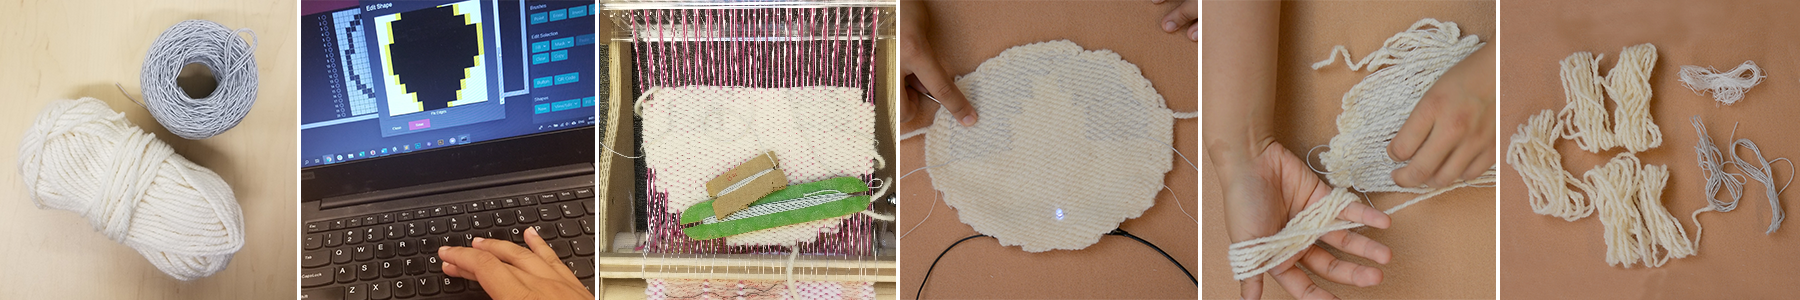
\includegraphics[width=\linewidth]{figs/UF_teaser.png}
	\caption[The lifecycle of a designed-for-disassembly e-textile component.]{
        The lifecycle of a designed-for-disassembly e-textile component (left to right): 1) Raw materials of conductive and non-conductive yarn. 2) Software for designing the layout and shape of components 3) Weaving/fabrication using an easy-to-disassemble technique developed in this work. 4) Testing the textile's electronic functionality. 5) Unravelling the textile to reclaim yarn. 6) Re-harvested yarn, ready to reuse.
    }
    \label{fig:teaser}

\end{figure}

% The project that would become Unfabricate started with a trip to the thrift store because I had recently learned about recycling yarn from old sweaters. The practice struck me as an example of something that was possible with textiles, but not with our current electronics. My crafting instincts kicked in, and I had to try it myself. As I practiced unravelling sweaters, I also learned how to select the garments that were easier to disassemble, and honed my untangling skills. There was a lot of untangling. 

Fittingly, as craft led me to deconstruct as part of the design process, it also led me to deconstruct my notions of technology in order to design e-textiles.
Having the language of coproduction that questioned how designers positioned (and privileged) knowledge from electronics vs. knowledge from textiles, I realized that this wisdom of textiles was most visible in mundane, often-ignored locations outside of the purview of "novel" technology. There were several features of textiles which I took for granted, but upon further reflection, these were features that would be difficult to achieve in the current electronic hardware paradigm. 
% The most striking feature to me was that textiles were easily disassembled. 
Notably, textiles can be mended to prolong their life, cut up to repurpose for scraps, and some can be unravelled to reuse their raw materials. I would personally love to see my electronic devices support any of these disassembly actions. It was something that I wanted to see in my future smart textile objects: to be able to unravel a smart garment or other device when it was no longer useful, then to be able to make something else with the yarn. Furthermore, I envisioned that this affordance was a default of future e-textiles, so that the technology actively participated in a sustainable world by recycling products and recirculating electronic materials as a crucial part of industrial activities. The ensuing design inquiry into designing smart textiles for disassembly led me to develop a new woven structure, modify the looms I used, and extend AdaCAD -- a proof-of-concept systemic retooling that resulted in a woven smart textile which I then fully unravelled. (Fig. 7)

% \section{Sensitization to a Coproductive Ecosystem}

%A tactic found in slow fashion, as well as throughout craft history when necessitated by economics, is to reclaim yarn from existing garments, such as knitted sweaters from a thrift store. For instance, knitters in the Great Depression would unravel handknits that were less used to avoid buying new yarn [18]. We turn to these practices to investigate an existing site of disassembly and reuse in textiles, which ties into a larger ecosystem of waste management and recycling around the globe. This project, eventually taking the name Unfabricate, started at a local thrift store. 

%Following tutorials from other crafters who reclaimed yarn from thrift store sweaters (some even sell the reclaimed yarn as a business) [158], I familiarized myself with features of knitted items that made them possible to unravel for usable amounts of yarn. I went to the thrift store to understand, from an embodied perspective, the process of both selecting and unraveling a pre-made garment. At the thrift store, we could see that many knitted garments would be unsuitable for unravelling. While the aforementioned properties of knit fabric (e.g. long continuous yarn in a slipknot) should generally result in more efficient unravelling than woven, the rest of the garment fabrication process can affect the yield of usable yarn. This is because knitwear manufacturing is divided into two main categories. 1) cut-and-sew, where a large rectangular swath of fabric is machine-knitted, then cut into pattern pieces and sewn together; and 2) fully-fashioned, where pieces are knitted with shaping and seamed without cutting. A third emergent category is whole garment knitting, a newer method where the garment is knitted in one piece.  Most of the garments in the thrift store (and produced internationally) are cut-and-sew and, as thus, our first challenge was spotting fully-fashioned knitwear, as these garments would produce the most long, usable lengths of yarn.

%Once we chose a garment to unravel, this element of reverse engineering and speculating on the garment's fabrication continued. For instance, the garment in Figure 8 was fully fashioned. To obtain the maximal amount of yarn from the knit, we needed to understand the order in which pieces were joined together and then, reverse when unraveling. This required analyzing the structure and "reading" its method of fabrication prior to unwinding. When cutting the seams to unpiece the knit, we found it easier to not only cut the seams in the reverse order of how they had been created, but also to reverse the direction of the seam and start cutting at its last stitch. My hand knitting experience helped me intuit these details of fabrication. After unraveling the garment, I washed and wound the yarn into looped bundles to return the yarn to a ready-to-use condition.

%After unravelling multiple garments with different yarns and construction details, we found some key principles for minimizing time and maximizing reclaimed material which would inform designing other textiles for disassembly:
%One needs to understand the order of the fabrication steps that created the knit. Like cutting along the grain of wood, rather than against, unravelling a knit is easier when the order of fabrication steps are reversed exactly. To support disassembly, designers should make the disassembly instructions clearly "readable" in their structure.

%At fabrication time, designers should cut the material as few times as possible to maximize the total amount of yarn that can be harvested from deconstruction.
%We also speculated that certain design tactics within knitting systems could aid unravelling and reclamation.
%Shape the pieces as they are fabricated so they do not have to be cut for sewing.
%Design the garment to use fewer but larger pieces to minimize the number of cuts in the yarn.
%If using multiple yarns, keep the contrasting yarns in contiguous areas to also minimize the number of cuts in each yarn.

% Discovering the techniques and hands of other makers gave us a poetic sense of satisfaction in returning the yarn to an "original" or blank state. As one takes apart the garment, its creation story is replayed rather than erased. While we understood the affordances of textiles to unravel, our sensitization process made us appreciate more the reflective value of unraveling and the unique capability of yarn to store its own history. 

% \section{Retooling Woven Smart Textiles for Disassembly}

% With disassembly as an inspiring site of coproduction as well as an intriguing design prompt, I began to retool elements of smart textiles weaving to translate the lessons in disassembly across crafts. In knitting, I had observed that the structure of a knitted fabric, based on loops and continuous slipknots, fundamentally made the process friendly to disassembly. Using these parameters, I conducted a series of experiments with modifying a woven fabric's structure to also incorporate continuous yarns, and ultimately looped yarns, as illustrated in Fig. 10.

% In order to achieve the modified woven structure on a larger piece, I found that I also had to modify my weaving hardware. I used a tabletop loom, as the next size up from a handheld pin loom. The modified structure's looped warp yarns had to be secured in both the front and back of the loom (see Fig. 13). This loom modification has precedent in the history of weaving, as velvet weavers during the Italian Renaissance would achieve their complex structures (which required multiple warp yarns on top of a basic ground warp) by hanging individual spools of additional yarn on the back of the loom [145].

% The final design was a circular woven piece, using the paired warp loop structure to make disassembly possible, as well as conductive yarn in a semi-circular arc shape that could sense a user's analog input. With tongue in cheek, we named it the "Smart Circle". (Fig. 14) The prototype's electrical function is equivalent to a potentiometer or variable resistor, but the textile form suggests applications for a soft dial or knob input, or perhaps a stroke-based interface to be worn on a shoulder. The Smart Circle was indeed unravelled and reclaimed for its yarn as shown back in Fig. 7.

% We closed our exploration of designing smart textiles for disassembly by presenting a provocation for designing more disassemble-able woven smart textiles, outlining three conceptual applications. Highlighting unique opportunities from disassembly, we proposed 1) how the designed-for-disassembly woven structure could create three-dimensional shapes; 2) how unravelling the yarn created the possibility of re-processing the yarn, renewing or altering its functional properties; and 3) taking advantage of unravelling in pieces to create a modular garment whose key components could be swapped and remade. In retrospect, while reflecting on this project to write my dissertation proposal, I came to understand disassembly as a coproduction, as the process was a coproduct of the original fabrication processes, the existing craft tools, and the human performing the disassembly that had to sensitize themself to the voices of these assembling agents.

% In summary, the Unfabricate project started with an example of coproduction (disassembly) as a provocation for a design inquiry, which became a retooling of smart textiles weaving to support disassembly. We started with a product, where the material has already been used, as a starting point for new tool ecosystems and sites. I then identified different components as targets of retooling: the craft structure, software design tools, and fabrication hardware. The end result was a proof-of-concept system that was a coproductive retooling, albeit not explicitly referencing either concept. By attending to coproduction's stance on differences in privilege/power between bodies of knowledge, I was able to take an activist stance on honoring textiles knowledge and prioritizing it equitably in smart textiles design. 


% Smart textiles development is combining computing and textile technologies to create tactile, functional objects such as smart garments, soft medical devices, and space suits. %With the ubiquity of both computers and textiles in society, design opportunities for smart textile applications are everywhere. 
% However, the field also combines the massive waste streams of both the digital electronics and textiles industries. The following work explores how HCI researchers might be poised to address sustainability and waste in future smart textiles development through interventions at design time.  Specifically, we perform a design inquiry into techniques and practices for reclaiming and reusing smart textiles materials and explore how such techniques can be integrated into smart textiles design tools. Beginning with a practice in sustainable or ``slow" fashion, unravelling a garment into yarn, the suite of explorations titled ``Unfabricate" probes values of time and labor in crafting a garment; speculates how a smart textile garment may be designed with reuse in mind; and imagines how electronic and textile components may be given new life in novel uses.

\section{Why Design E-Textiles for Disassembly?}

The emergent field of smart textiles is predicted to be a \$5.5bn global industry by 2025 \cite{research_global_2019}. This field describes research embedding fabrics with circuitry or otherwise ``smart" materials at the yarn level. As the synthesis of both textiles and electronics, such an industry could compound the two's already-massive waste streams \cite{noauthor_smart_2012, circular_fashion, WEARSustain}. Firstly, textile production continues to be one of the most wasteful and polluting industries in the world. The National Resources Defense Council describes textile mills as producing 20\% of the world's industrial water pollution (through processes of dyeing, washing, etc.) \cite{noauthor_encourage_nodate} and the Ellen MacArthur Foundation reports that \$500bn is lost each year on "underused clothes and the lack of recycling" \cite{circular_fashion}. Secondly, the global electronics industry generates nearly 50 million metric tons of electronics waste or ``e-waste" annually \cite{rifat_breaking_2019}. As another major waste stream, the problem of e-waste has created secondary problems of regulating, transporting, and properly disposing of it, exacerbating inequities between developed and developing countries as the latter disproportionately receives e-waste to process \cite{Zhang:2011:DAU:2347504.2347511, raghavan_means_2017}. We expect these problems to compound with the introduction of custom electronics embedded into textile structures.

While concerning, smart textiles also present some interesting properties to support disassembly and recycling that are different from traditional electronics manufacturing. In smart textiles, circuitry is largely woven or knitted into a fabric structure, allowing us to envision ecosystems of adhesive-less circuitry, where prototypes or post-use objects can be unraveled and separated to re-harvest constituent materials~\cite{zysset_weaving_2010}. \textbf{From these structures, we can envision modes of disassembling or mending smart textiles, just as people can (and do) disassemble some garments that have been worn out or outgrown.} Unfabricate considers not only how these processes might take place, but if there are optimizations that HCI designers and developers could make at the time of design and fabrication to integrate disassembly and reuse into the smart textiles lifecycle. As such, we aim to connect communities discussing computational design and fabrication with those addressing sustainability through disassembly and reuse.

Drawing from sustainability tactics in fashion and handcraft, as well as design-for-disassembly practices \cite{webster_dfd,circular_disassembly}, this project investigates problems of sustainability and scalability in smart textiles by probing the variety of design possibilities for disassemble-able smart textiles. Our project begins with an inquiry into locating and unraveling existing garments, focusing on identifying techniques that assist in this process. We took our findings from unraveling knitwear to re-envision smart weaving techniques that might offer similar ease of unraveling, developing a technique of "warp overlaying" that increases the yield of usable yarn harvested from woven prototypes. We then concertized our approach in the form of an extension to AdaCAD, a smart textiles design tool, and tested it by creating (and unraveling) a woven potentiometer (Fig.~\ref{fig:teaser}). Throughout this process, we saw a suite of possible interventions throughout the weaving cycle to support disassembly, including hardware modifications on the loom machinery and software modifications in CAD. Specifically, we discovered how software could be aware of material constraints while working within current representational formats. As such, the practice of tool-building led us to broader speculation on what tools and systems could both support and incentivize investment in recyclable smart textiles. We share descriptions of our process and the techniques we developed to inspire future directions for HCI design research into smart textiles sustainability.
 
 %We draw from practices of unraveling which already exist, but have not yet been explored within the domain of computational fabrication for smart textiles. \todo{Speculate on larger visions. Add something of the reason HCI researchers can be useful in addressing this (i.e. it's not just a manufacturing/social problem).} As a field that encompasses many human-technology interactions and relationships, HCI is well-suited to exploring how both humans, devices, manufacturing, and other sociotechnical factors might have to adapt for a world of sustainable technology.

%Describe our approach and outlining our "contributions" to the field: This is a provocation for others to explore this research space with an idea for a way you could go about it.} We undertook a method of sensitization, variation within the domain, and lateral exploration to produce a prototype of a designed-for-disassembly smart textile component. Along the way, we uncovered several possible interventions in software, hardware, and the overall design process. 

%We began sensitization with a trip to the thrift store, a widely-familiar setting for reuse and reclamation; continued with selecting garments for disassembly in knitwear. In this stage, we learned about methods for unravelling knitwear into usable yarn and found possible design principles for disassembly/reusability. We then transitioned from knitwear to designing weaving for disassembly to test these principles further, finding that we could vary the woven structure and established techniques to facilitate disassembly. In an exploratory implementation, we saw a suite of possible interventions throughout the weaving process to create a disassemble-able smart textile, including hardware modifications in the loom machinery and software modifications in CAD to be more aware of material constraints and working within current representational formats.

\textbf{Our primary contribution is demonstrating how computational design can bridge developments across disciplines such as craft, textiles engineering, and materials science to advance sustainability.} Specifically, we want to bring researchers designing computational design tools into the existing conversations of design for disassembly and sustainable textiles. While our process yields insights through tool building, we acknowledge that capitalism, politics, and other sociological factors also make textiles unsustainable (e.g. we do not have sustainability problems \textit{because} of our tools and machines alone). Yet, we see tools as a site for making unraveling and reuse processes more available to users, enabling their own inquiry, exploration, and innovations. More interestingly, we see this as a place where HCI practitioners can make a meaningful difference within broader economic and social flows.  

%%%%%%%%%%%%%%%%%%%%%%%% BACKGROUND %%%%%%%%%%%%%%%%%%%%%%%%%%%%%
\section{Background: Textiles and Sustainability}
Our research addresses ongoing conversations in HCI about smart textiles development, sustainable design, and computer-aided design and manufacturing tools. Furthermore, our work connects related design work in other disciplines, such as fashion and industrial textiles. We look to specific terminology, practices, and programs within fashion and textiles (from both craft and industry perspectives) to inspire our approach.  While some argue that the integration of circuitry and computational abilities into garments can extend their lifespan by dynamically "updating" to meet current trends  \cite{ivan_keynote} or perhaps becoming reflective artifacts containing aspects of our histories (through techniques such as \cite{rosner_spyn:_2008}), we look to offer another perspective that focuses, and perhaps extends, the lifespan of the \textit{materials} as opposed to the artifacts---thus allowing artifacts to be shaped, unshaped, and reshaped into novel forms. In this sense, we draw inspiration from a growing "design-for-disassembly" movement that considers how designers can shape how their artifacts are used (and reused) \cite{webster_dfd, circular_disassembly}.

\subsection{Fabricating Sustainable Textiles}
Within the domains of fashion and textile design, concerns for sustainability have become manifest in programs such as "slow fashion" \cite{phelan_what_2017} and "circular fashion" \cite{circular_fashion}. Practitioners approach sustainability and slowness from multiple backgrounds, ranging from couture designers \cite{piper_crafting_2015} and fashion scholars \cite{fletcher_sustainability_2014, fletcher_craft_2016}, to professional craftspeople \cite{essen_easysupp_2016, unravellingclub} and self-taught makers \cite{ravelry_thriftyknitters}. In a handbook on sustainability and fashion, contributors call for research agendas that consider the systemic unsustainability of the modern textile industry and reframe the identities of consumer, production worker, and other stakeholders \cite{fletcher_sustainability_2014}.

Some work in this domain envisions new manufacturing infrastructures for textiles that mimic the visions offered of additive manufacturing but focusing on soft goods. Specifically, Pamela Liou, a designer and technologist, envisioned a new form of cottage industry supported through an open-source tabletop Jacquard loom called Doti \cite{liou_doti:_2015}. This is mirrored in companies like WOVNS that focus on fabricating small runs of user designed products \cite{wovns}. Along with other technologies like the Kniterate, we are beginning to see workflows where users can print textile products on demand \cite{kniterate}. 

In parallel to the growth of "grass-roots" textile manufacturing equipment, new software protocols are being developed to develop fully shaped artifacts based on digital inputs \cite{mccann_compiler_2016, albaugh_digital_2019}. Such work contributes to our agenda by ensuring shapes are made from long continuous lengths of yarn, as opposed to separate panels that are cut to shape and bound with sewing machines. Our work contributes a perspective that specifically focuses on weaving, a process that does not yet lend itself to easy unravel-ability in the same way as knitted objects. 

Weaving is one of the most common textile production methods (for denim, upholstery, etc) whose structures offer specific supports for smart textiles development \cite{devendorf_adapting_2019, poupyrev_project_2016, worbin_designing_2010, orth_fabric_1998, mikkonen_weaving_2015}. The exploration of woven smart textiles is further supported by the availability of hardware such as the TC2 digital jacquard loom \cite{norway_tc2_nodate}, which specifically offers industrial style weaving supports to prototype and small-run makers. In previous work, we have explored custom software for smart textiles design by creating AdaCAD, a program that builds upon weaving's available notations and techniques \cite{friske_adacad:_2019} (a full summary of such notation can be found there).

\begin{figure}
    \centering
    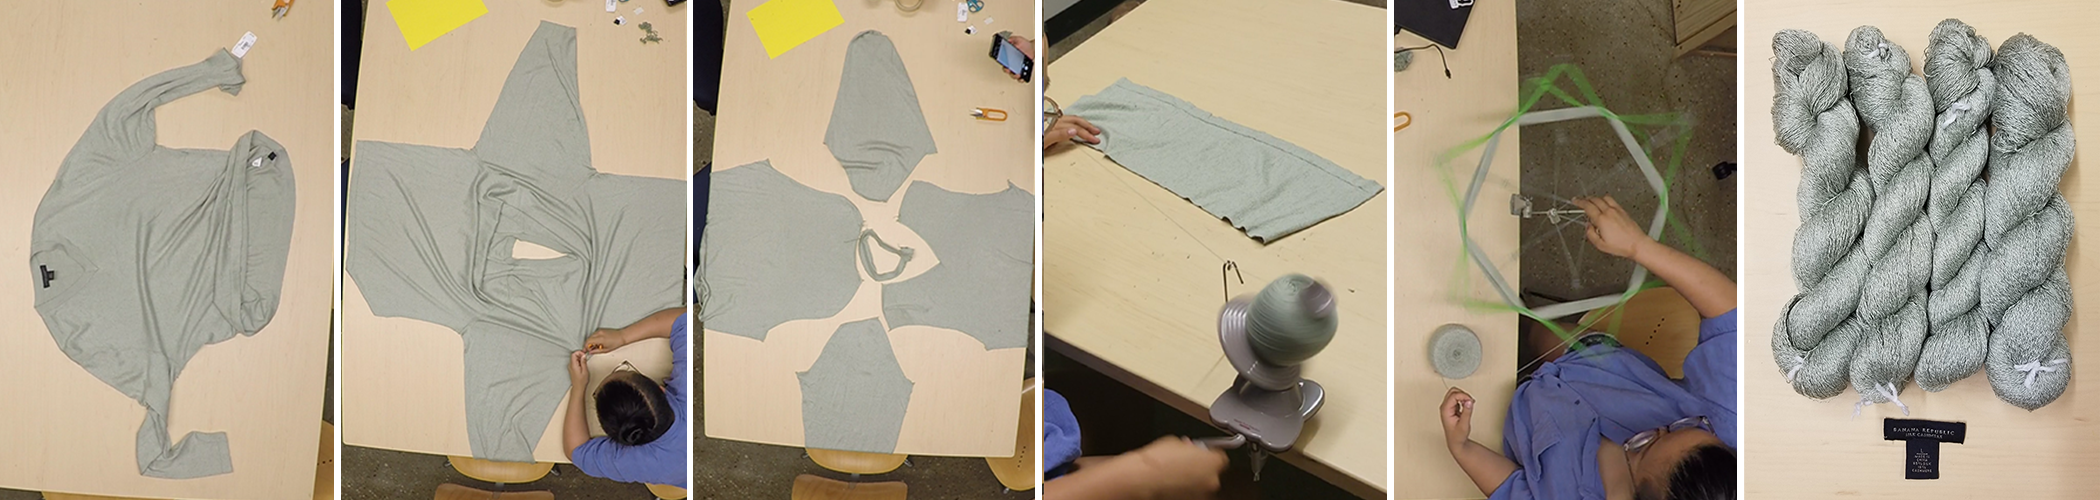
\includegraphics[width=\linewidth]{figs/UF_unravelling_6panels.png}
    \caption[The process of unravelling a knit garment and reclaiming its yarn.]{The process of unravelling a knit garment and reclaiming its yarn. a) The initial garment. b) Separating the first set of seams. c) The garment pieces fully separated. d) Unravelling each piece with the help of a yarn winder. e) Winding the unravelled yarn into loops to prevent tangles. f) The reclaimed yarn shown, after washing, with the original garment label.}
    \label{fig:unravelProcess}
\end{figure}

\subsection{Approaches to Sustainability and Reuse in HCI}

For the past two decades, HCI's interest in supporting sustainable innovation has grown dramatically. This includes projects that target behavior change on an individual level \cite{disalvo_mapping_2010, dourish_hci_2010}, bring greater awareness to ones environment in terms of pollutants \cite{kim_wearair:_2010, da_costa_interspecies_nodate, aoki_vehicle_2009}, critical reflection on how HCI plays into existing consumerist processes~\cite{blevis_sustainable_2007, pan_fashion_2014,raghavan_means_2017}, or support social practices of sustainability such as urban foraging \cite{disalvo_fruit_2017}. More recently, and joined under a broader theoretical framework of the Anthropocene, researchers have looked to broader methods as platforms for sustainable behavior. These include approaches that bring users in greater physical contact with the environment \cite{liu_design_nodate, kuznetsov_nurturing_2011, light_design_2017} or approaches that question the fundamental orientation of HCI as on that is focused on "ease of use" \cite{light_design_2017} to make space for new forms of perhaps challenging but otherwise meaningful and neccessary action \cite{devendorf_hci-amusement_2019, Dew:2018:MWL:3232617.3232626, Dew:2019:DWS:3322276.3322320}.

Research specifically focusing on practices of repair and reuse \cite{jackson_repair_2012, Dew:2019:DWS:3322276.3322320, Dew:2018:LWC:3173574.3174159, Wyche_postcolonialphone, Wakkary_greendesignfiction, Tsaknaki_thingsfallapart} offer a productive intersection of sustainable-thinking and noticing through hands-on practices with broken or otherwise outmoded materials. This has taken the form of studies of "everyday design" \cite{Wakkary:2009:SIC:1518701.1518761, Maestri:2011:URC:2069618.2069633}, through critical ``deconstruction" activities \cite{Murer:2018:MTA:3196709.3196806, Murer:2015:DID:2882850.2882860, Murer:2017:UDE:3024969.3024993}
, and by approaching artistic practices of reuse through attending to the "life" of that which is being reused \cite{jackson_breakdown_2014}. We draw from these projects to both become sensitive to what the practice of reuse entails while also exploring how one might "optimize" a design to make such practices more accessible and available to broad audience. In this way, we shift our focus from repairing artifacts whose forms are already set and made, to focusing on how we might make those forms to suggest repair from the beginning of their design. In this sense, we draw out work in line that explores fabrication with "salvage" \cite{Dew:2019:DWS:3322276.3322320} or otherwise spare materials \cite{devendorf_being_2015,KovacsTrussFormer}. 

%\subsection*{Computation Design Tools and Reuse}
%Most CAD tools are created for the production of new items independent of attending to their full lifespan or how they might be "unmade." Other CAD tools emphasize making with found materials (Remind Laura to send these), which lend themselves to appropriation through reuse. 

%--include Hudson and the other guy's interface for using found objects and inserting them into CAD drawings. Mueller's lego building cad and wireprint as an example of limiting materials usage at design time. 

%\begin{itemize}
%\item Reusing/Embedding Everyday Objects into 3D prints for new functions: %https://dl.acm.org/citation.cfm?id=3173736, https://dl.acm.org/citation.cfm?id=3173637
%\item Sustainable in the Sense that it Gives sense of shape without use of materials: %https://dl.acm.org/citation.cfm?id=2647359; https://dl.acm.org/citation.cfm?id=2574779, %https://dl.acm.org/citation.cfm?id=3025699,
%\item Some 3D print fashion stuff aiming at zero waste: %https://link.springer.com/article/10.1186/s40691-018-0152-2
%\end{itemize}

%More general studies of mending:
%https://dl.acm.org/citation.cfm?id=2479674
%https://dl.acm.org/citation.cfm?id=2820021

%This track (Kristin Dew) Seems most relevant - take a good look at what she sites, there are likely to be more in there: 
%https://dl.acm.org/citation.cfm?id=3232626
%https://dl.acm.org/citation.cfm?id=3322320
%https://dl.acm.org/citation.cfm?id=3232626

%Some e-waste specific reuse: 
%https://dl.acm.org/citation.cfm?id=1979292

%Practices of reuse in textiles - 
%Shedding and Shoddy - https://www.press.uchicago.edu/ucp/books/book/chicago/S/bo24045083.html

%Extending Lifespan through Imbuing with memories:
%https://dl.acm.org/citation.cfm?id=1753691

%Slow Design, 
%https://dl.acm.org/citation.cfm?id=2318088

%Here we can survey the tools available for textile design, introduce AdaCAD and how we are integrating this into AdaCAD....
%\todo{introduce drafts here}

\subsection{Unravel-ability of Knitted and Woven Garments}
% keep this brief, but give a quick introduction to why it matters.

Knitting and weaving are two distinct and common methods of industrial textile production that both form fabric by manipulating yarn. In knitting, a single yarn forms interlocked loops which comprise the fabric, essentially creating a complex slipknot (Figure~\ref{fig:cutcont_knitweave}). A knit garment could be made using just one continuous length of yarn, which is why knit garments lend themselves more readily to unraveling. In weaving, two yarn systems are required: \emph{warp} yarns along one axis, and \emph{weft} yarns on the perpendicular axis. The warp is set up on the machine (\emph{warping} the loom) prior to weaving, then the weft is inserted perpendicular to the warp, travelling over and under the warp to create fabric through these interlacements. This process is more difficult to unravel, because each warp is a discrete, rather than continuous piece of yarn. Additionally, several practices of assembling woven fabrics into garments and products make additional cuts, and thus, reduce the number of usable lengths of yarn that can be extracted.
 
Industrialized weaving further cuts the yarn. Many automated factory looms use a ``rapier" mechanism that cuts the yarn after every row in order to speed up weaving \cite{engineers_complete_2017}. This mechanism represents how weaving manufacturing infrastructure is optimized for throughput, to produce as much fabric as quickly as possible, which trades off disassembly as a consequence.


%%%%%%%%%%%%%%%%%%%%%%%% METHODS %%%%%%%%%%%%%%%%%%%%%%%%%%
\section{Methods and Approach}

This inquiry takes place in phases: 1) a ``sensitization activity" focused in disassembling existing knit textiles; 2) applying our learnings from disassembly to inspire new structures and hardware modifications to produce disassemble-able \textit{woven} structures; 3) and encoding these practices into a design tool to both demonstrate the feasibility of this feature as a design default while also inspiring future visions of technical intervention to promote and support reharvesting materials. These strategies represent a combination of several research through design methods in HCI. The idea of sensitizing oneself to a design space combines ideas from design anthropology \cite{smith_design_2016} and reflective design \cite{sengers_reflective_2005}, immersing oneself as a designer and observer into an environment to understand how it took on a particular form.

In our case, the environment of interest was the ecology (or lack thereof) that had been built around disassembling and reusing textiles. Targeting these values with probes in the form of technical experiments, we situated our role in the ecosystem as consumers and makers of textile goods, but not manufacturers~\cite{gaver_design:_1999, gaver_what_2012}. 

% Account for your own expertise in knitting and weaving and how this positions your exploration from a unique perspective. 
As an experienced knitter and weaver who learned these fiber crafts alongside traditional engineering and science subjects, Wu was uniquely positioned for this exploration. Leveraging their expertise in handcraft, our work seeks to emphasize embodied making processes and exploring through craft~\cite{ingold_making:_2013}. Our sensitization to values in disassembly and in the \emph{hand} as a metaphor for the unseen, unrecognized labor in dealing with waste \cite{rifat_breaking_2019} led us to use the created tools ourselves in the vein of autobiographical design~\cite{neustaedter_autobiographical_2012, desjardins_living_2016, desjardins_revealing_2018}. Taking a page from practices of design fiction~\cite{kirsh_how_2011, blythe_pastiche_2004}, workbooks~\cite{gaver_making_2011}, and HCI amusements~\cite{devendorf_hci-amusement_2019}, we offer three concepts or design sketches for future systems intended to spark the imagination of others working HCI to consider default settings for sustainable manufacturing in textiles and beyond.

%\todo{The next paragraph can outline the limitations when we think of this at scale but cite articles that talk about fiction and speculation as productive. Basically, we are turning, again, to indivdiuals as a first step because we don't yet know enough about industrial manufacturing to make strong claims about their workflows. While this is limited, we hope it reveals themes and concepts that can inspire more work in the domain, specifically the idea that we can design for deconstruction from the forefront. }
Our later phases of work in producing a design artifact and describing the creative possibilities it inspired are speculative in nature. We acknowledge the limitations of our built prototypes as a single research group, yet the narrative power of design fiction from a small cohort of authors can compel larger groups to envision new futures \cite{dunne_speculative_2013}. In future work, We hope to continue this model of experimental units and creative exercises in order draw more connections between different technical and creative practices.
%%%%%%%%%%%%%%%%%%%%%%%% PROCESS %%%%%%%%%%%%%%%%%%%%%%%%%%

\section{Process}
% Give really high level overview and snippet of outcomes....
%This work began in knitting, and then transitioned to weaving. Smart textiles research includes many forms of textile manufacturing, so investigating a general design paradigm means that we have to look at more than one fabrication mode. How do things translate?
%I don't know if this paragraph brings me particular value

\subsection{Sensitization: Unravelling Procedures}
A tactic found in slow fashion, as well as throughout craft history when necessitated by economics, is to reclaim yarn from existing garments, such as knitted sweaters from a thrift store. For instance, knitters in the Great Depression would unravel handknits that were less used to avoid buying new yarn \cite{black_knitting:_2012}. We turn to these practices to investigate an existing site of disassembly and reuse in textiles, which tie into a larger ecosystem of waste management and recycling around the globe.

As a first step towards our study of unraveling, we sought to understand, from an embodied perspective, the process of both selecting and unraveling a pre-made garment. As such we took a trip to a thrift store to assess the availability of garments to unravel. At the thrift store, we could see that many knitted garments would be unsuitable for unravelling. While the aforementioned properties of knit fabric (e.g. long continuous yarn in a slipknot) should generally result in more efficient unravelling than woven, the rest of the garment fabrication process can affect the yield of usable yarn. This is because knitwear manufacturing is divided into two main categories. 1) \emph{cut and sew}, where a large rectangular swath of fabric is machine-knitted, then cut into pattern pieces and sewn together; and 2) \emph{fully fashioned}, where pieces are knitted with shaping and seamed without cutting. A third emergent category is \emph{whole garment knitting}, a newer method where the garment is knitted in one piece.  Most of the garments in the thrift store (and produced internationally) are cut and sew and, as thus, our first challenge was spotting fully fashioned knitwear, as these garments would produce the most long, usable lengths of yarn. 

Once we chose a garment to unravel, this element of reverse engineering and speculating on the garment's fabrication continued. For instance, the garment in Figure~\ref{fig:unravelProcess} was fully fashioned. To obtain the maximal amount of yarn from the knit, we needed to understand the order in which pieces were joined together and then, reverse when unraveling. This required analyzing the structure and "reading" its method of fabrication prior to unwinding. When cutting the seams to unpiece the knit, we found it easier to not only cut the seams in the reverse order of how they had been created, but also to reverse the direction of the seam and start cutting at its last stitch. Wu's extensive hand knitting experience helped them intuit these details of fabrication. After unraveling the garment, we washed and wound the yarn into looped bundles to return the yarn to a ready-to-use condition.

We continued to unravel eight garments of various yarn weights and materials. Most appeared to be commercially knit, while two of these garments appeared to be handknit. Both kinds of garments tended to follow similar templates for their construction order but different methods for seaming. %Commercially-produced knits use a ``linker" machine to quickly make evenly-stitched seams, which produces a distinct chained appearance. 
After unravelling multiple garments with different yarns and construction details, we found some key principles for minimizing time and maximizing reclaimed material which would inform our design tool: 

\begin{itemize}
    \item One needs to understand the order of the fabrication steps that created the knit. Like cutting along the grain of wood, rather than against, unravelling a knit is easier when the the order of fabrication steps are reversed exactly. To support disassembly, designers should make the disassembly instructions clearly "readable" in their structure.
    \item At fabrication time, designers should cut the material as few times as possible to maximize the total amount of yarn that can be harvested from deconstruction.
\end{itemize}

We also speculated that certain design tactics within knitting systems could aid unravelling and reclamation.
\begin{itemize}
    \item Shape the pieces as they are fabricated so they do not have to be cut for sewing.
    \item Design the garment to use fewer but larger pieces to minimize the number of cuts in the yarn.
    \item If using multiple yarns, keep the contrasting yarns in contiguous areas to also minimize the number of cuts in each yarn.
\end{itemize}

% might be nice to end here with some reflection on your experience - maybe a recognition of the many "hands" that shaped the machined garment in the first place?

Our experience in unravelling these knitted objects created a heightened awareness of the time and labor invested in their fabrication, as we put in additional time and labor to undo the fabrication. Before this work, we had the misconception that commercial knits were nearly fully automated. However, in attending to the details and variations in manufacturing in each garment, we clearly recognized the touch of many hands throughout the process. Knitting machines, even when computer-controlled, require extensive manual configuration to place each stitch in the machine, and may even require hand manipulation for certain shaping methods and seaming methods \cite{rowan_machineknitting}.

Discovering the techniques and hands of other makers gave us a poetic sense of satisfaction in returning the yarn to an "original" or blank state. As one takes apart the garment, its creation story is replayed rather than erased. While we understood the affordances of textiles to unravel, our sensitization process made us appreciate more of the reflective value of unraveling and the unique capability of yarn to store its own history. 

While not central to our research focus, we wanted to contribute our knowledge of useful unravelling to the community in the form of a zine and research video\footnote{http://sminliwu.github.io/projects/Unfabricate}. By choosing these formats rather than an online tutorial, we hope to foreground the non-procedural elements of unravelling and encourage reflection during this practice. Figure \ref{fig:unravelProcess} shows key frames from the research video, documenting the process from the initial garment to usable yarn.  

\subsection{Designing for Unravelling}

\subsubsection{From Knitting to Weaving}

% background of knitting vs. weaving
\begin{figure}
    \centering
    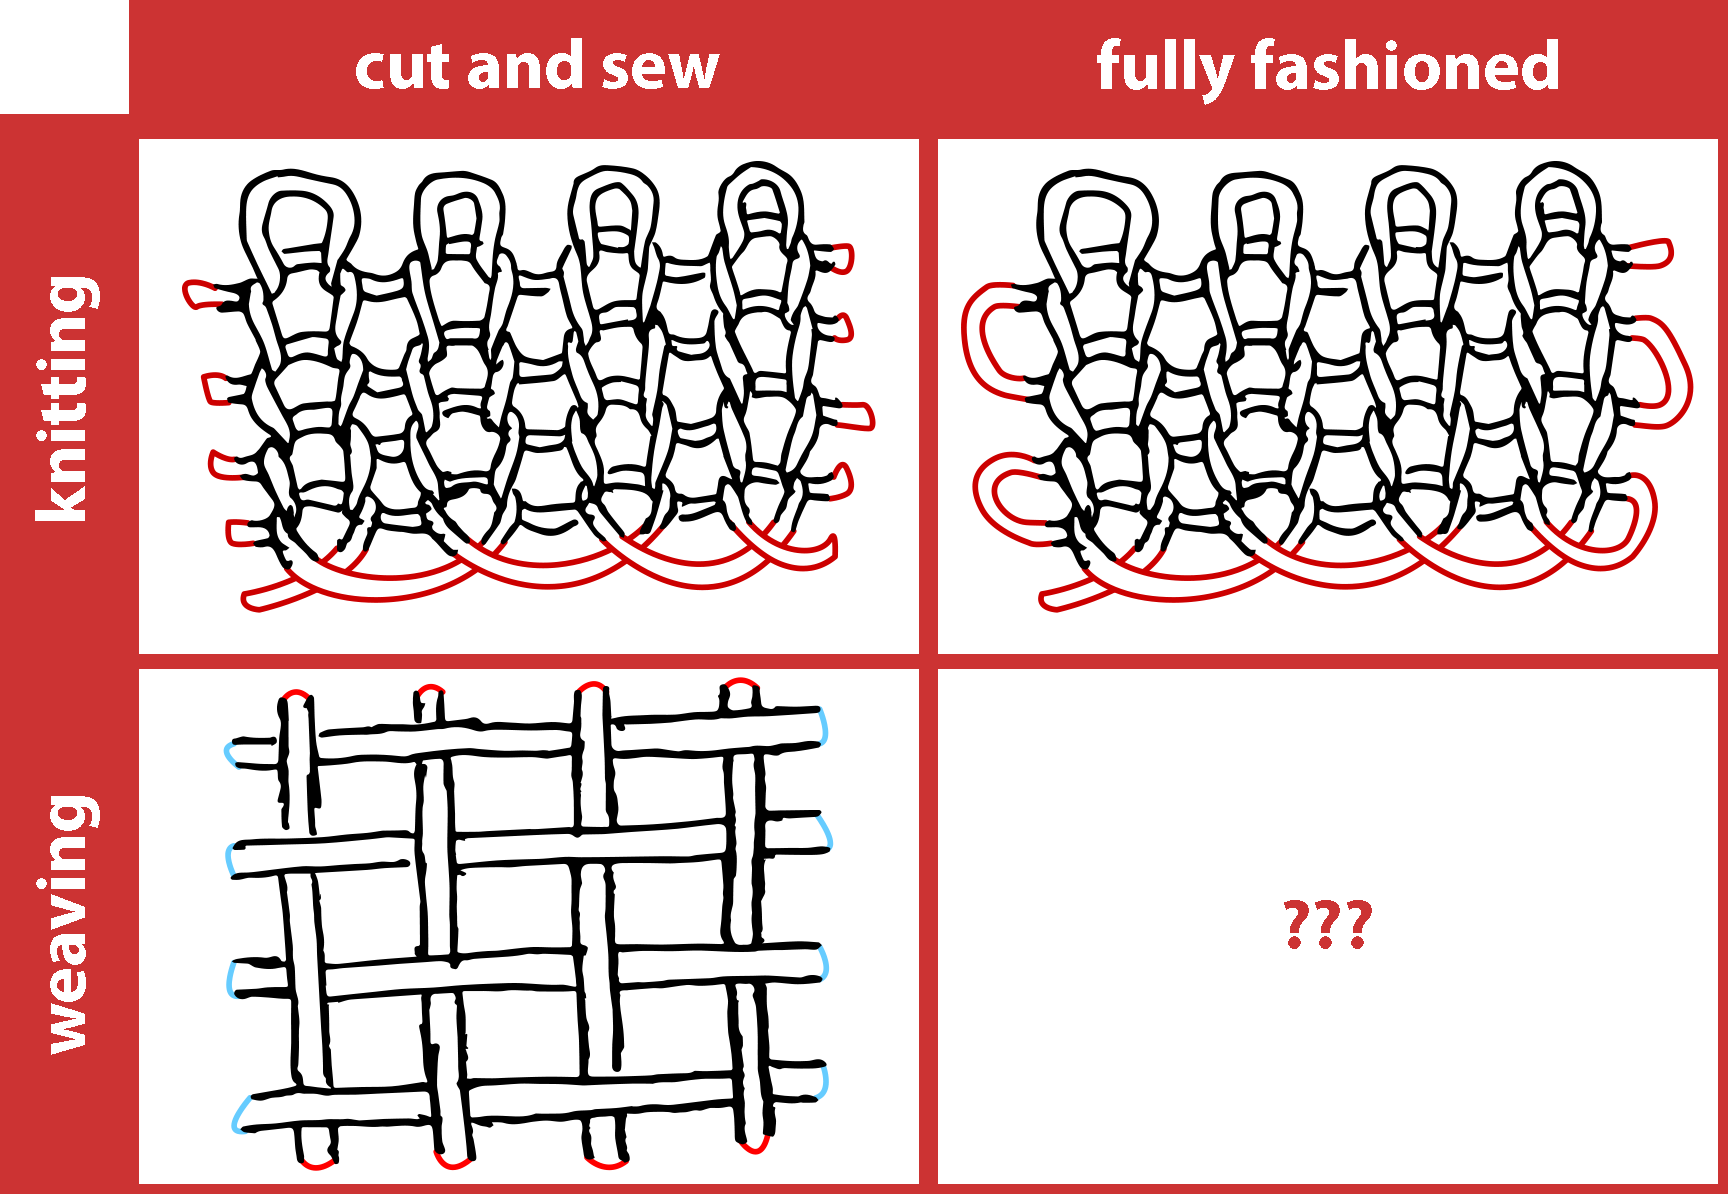
\includegraphics[width=\linewidth]{figs/UF_knitweave_cutff.png}
    \caption[Structural differences between knitting and weaving.]{Summary of structural differences between knitting and weaving. Cut and sew versus fully fashioned manufacturing treats the edges of pieces differently. The yarns remain continuous in fully-fashioned knitwear. No such equivalent exists in industrialized wovens.}
    \label{fig:cutcont_knitweave}
\end{figure}

From our sensitization exercise, we saw knitting as a design space that seems well suited to designed-for-disassembly smart textiles. However, the smart textiles field includes both knits and wovens, among other fabrication methods, which may each pose their own challenges to designing for disassembly. 
Unlike knits, wovens are nearly always manufactured via cut and sew. Furthermore, many industrial looms incorporate mechanisms (e.g. rapier, projectile) which cut the weft after every row. As a result, many wovens available to consumers are almost exclusive composed of short pieces of yarn that would be difficult to reuse. For a summary of cut-and-sew and fully fashioned in both knitting and weaving, see Figure~\ref{fig:cutcont_knitweave}.

\subsubsection{Shape Weaving}
In unravelling knits, we noticed some key features---continuous yarns and shaping---that enabled reclaiming usable materials from the finished object. What if wovens were designed with these features in mind to reduce waste not only during fabrication but in post-consumer stages? We began with looking to existing work in loom-shaped and fully fashioned woven garments to create shapes from continuous lengths of yarn.
 %switched to a more active voice here
Shape weaving describes a process where weft yarn is restricted to portions of the warp, rather than span the entire width of the loom. These pieces could then be cut off the loom and separated. However, this leaves loose ends in the warp which would then have to be secured to prevent fraying. Thus, we looked for methods and adaptations we could develop that would create continuous threads along the warp and the weft. In a series of technical experiments, we wove non-rectangular pieces while iterating on methods for securing the warp to preserve the shapes' edges, evaluating them on set-up/finishing times, potential wastage, and scalability. 

Industrial settings are indirectly designed against shape weaving, since all wefts including inlay and supplementary yarns travel from edge to edge. %Rapier looms even cut the weft yarn after every row. \todo{(cite)} 
This is likely to also be a manufacturing challenge for future woven smart textiles at scale, because circuitry favors continuous lengths of conductive yarn in narrow regions which may not span the width of the loom. With the advent of Jacquard looms for non-industrial settings, preparing a CAD file for weaving is becoming accessible to more single users, leading us to believe that there could be a broader space for experimentation in shape woven structures outside of formal production settings. 

\begin{figure}
    \centering
    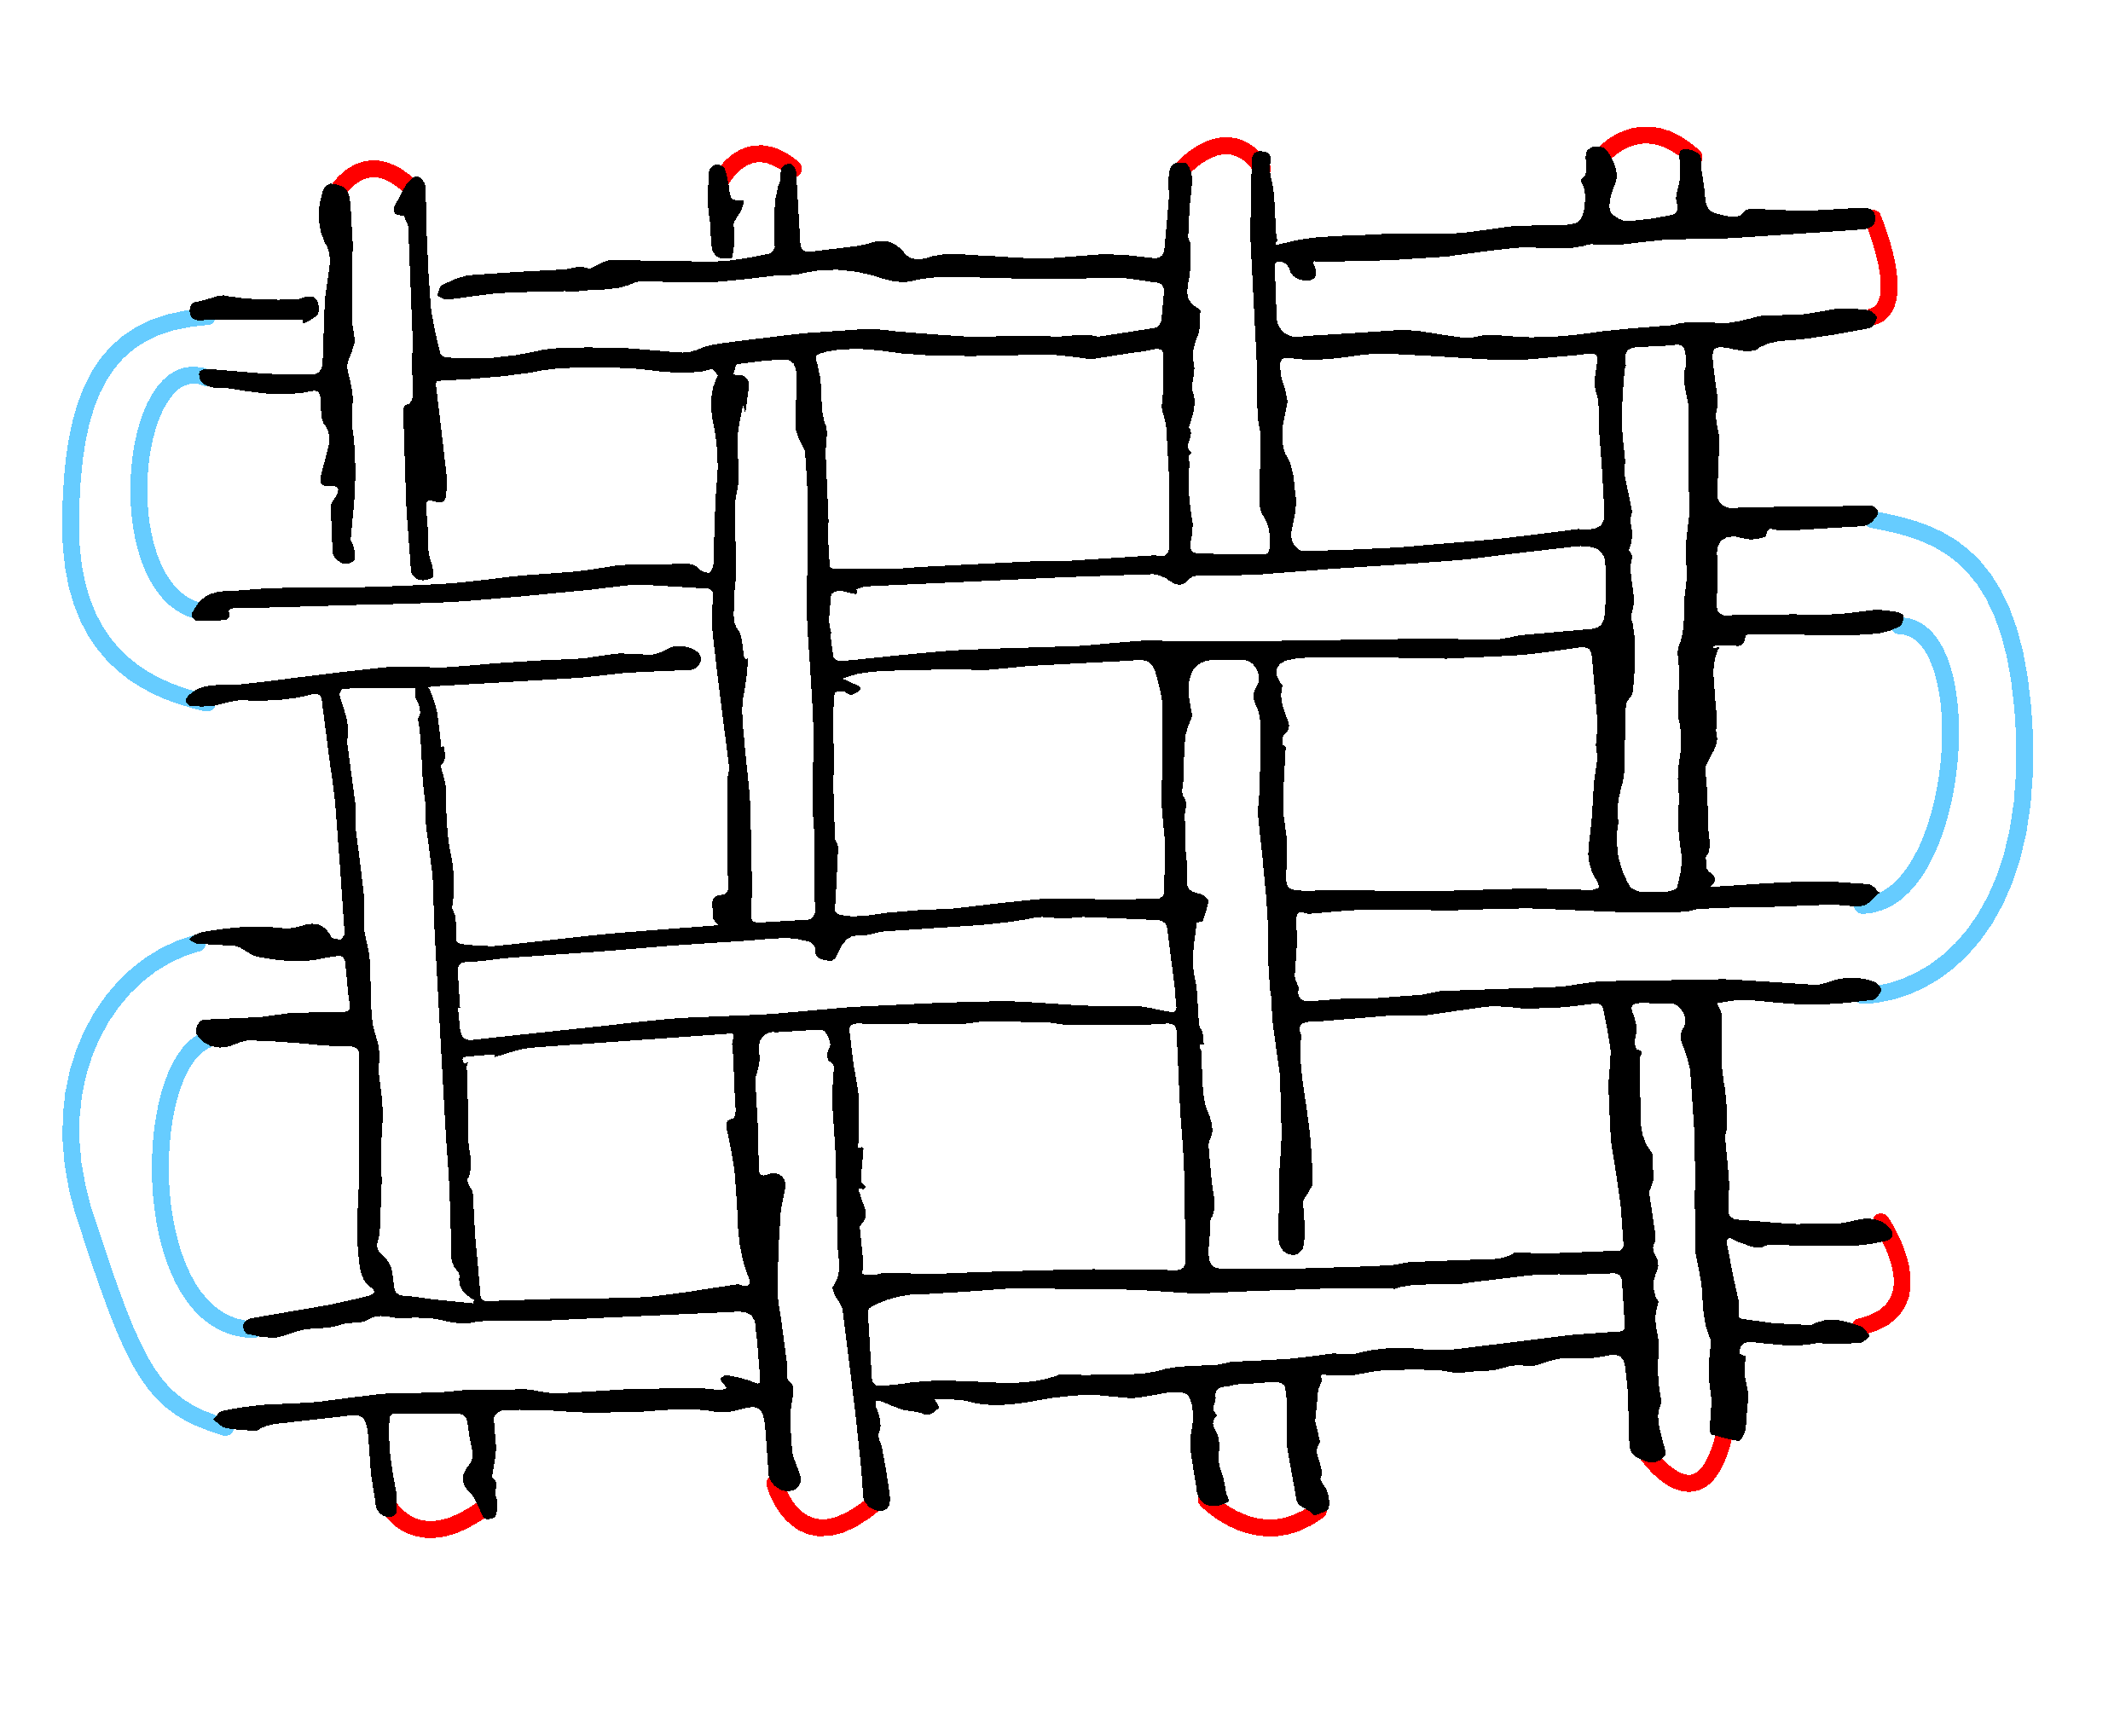
\includegraphics[width=0.3\linewidth]{figs/UF_weave_contweft.pdf}
    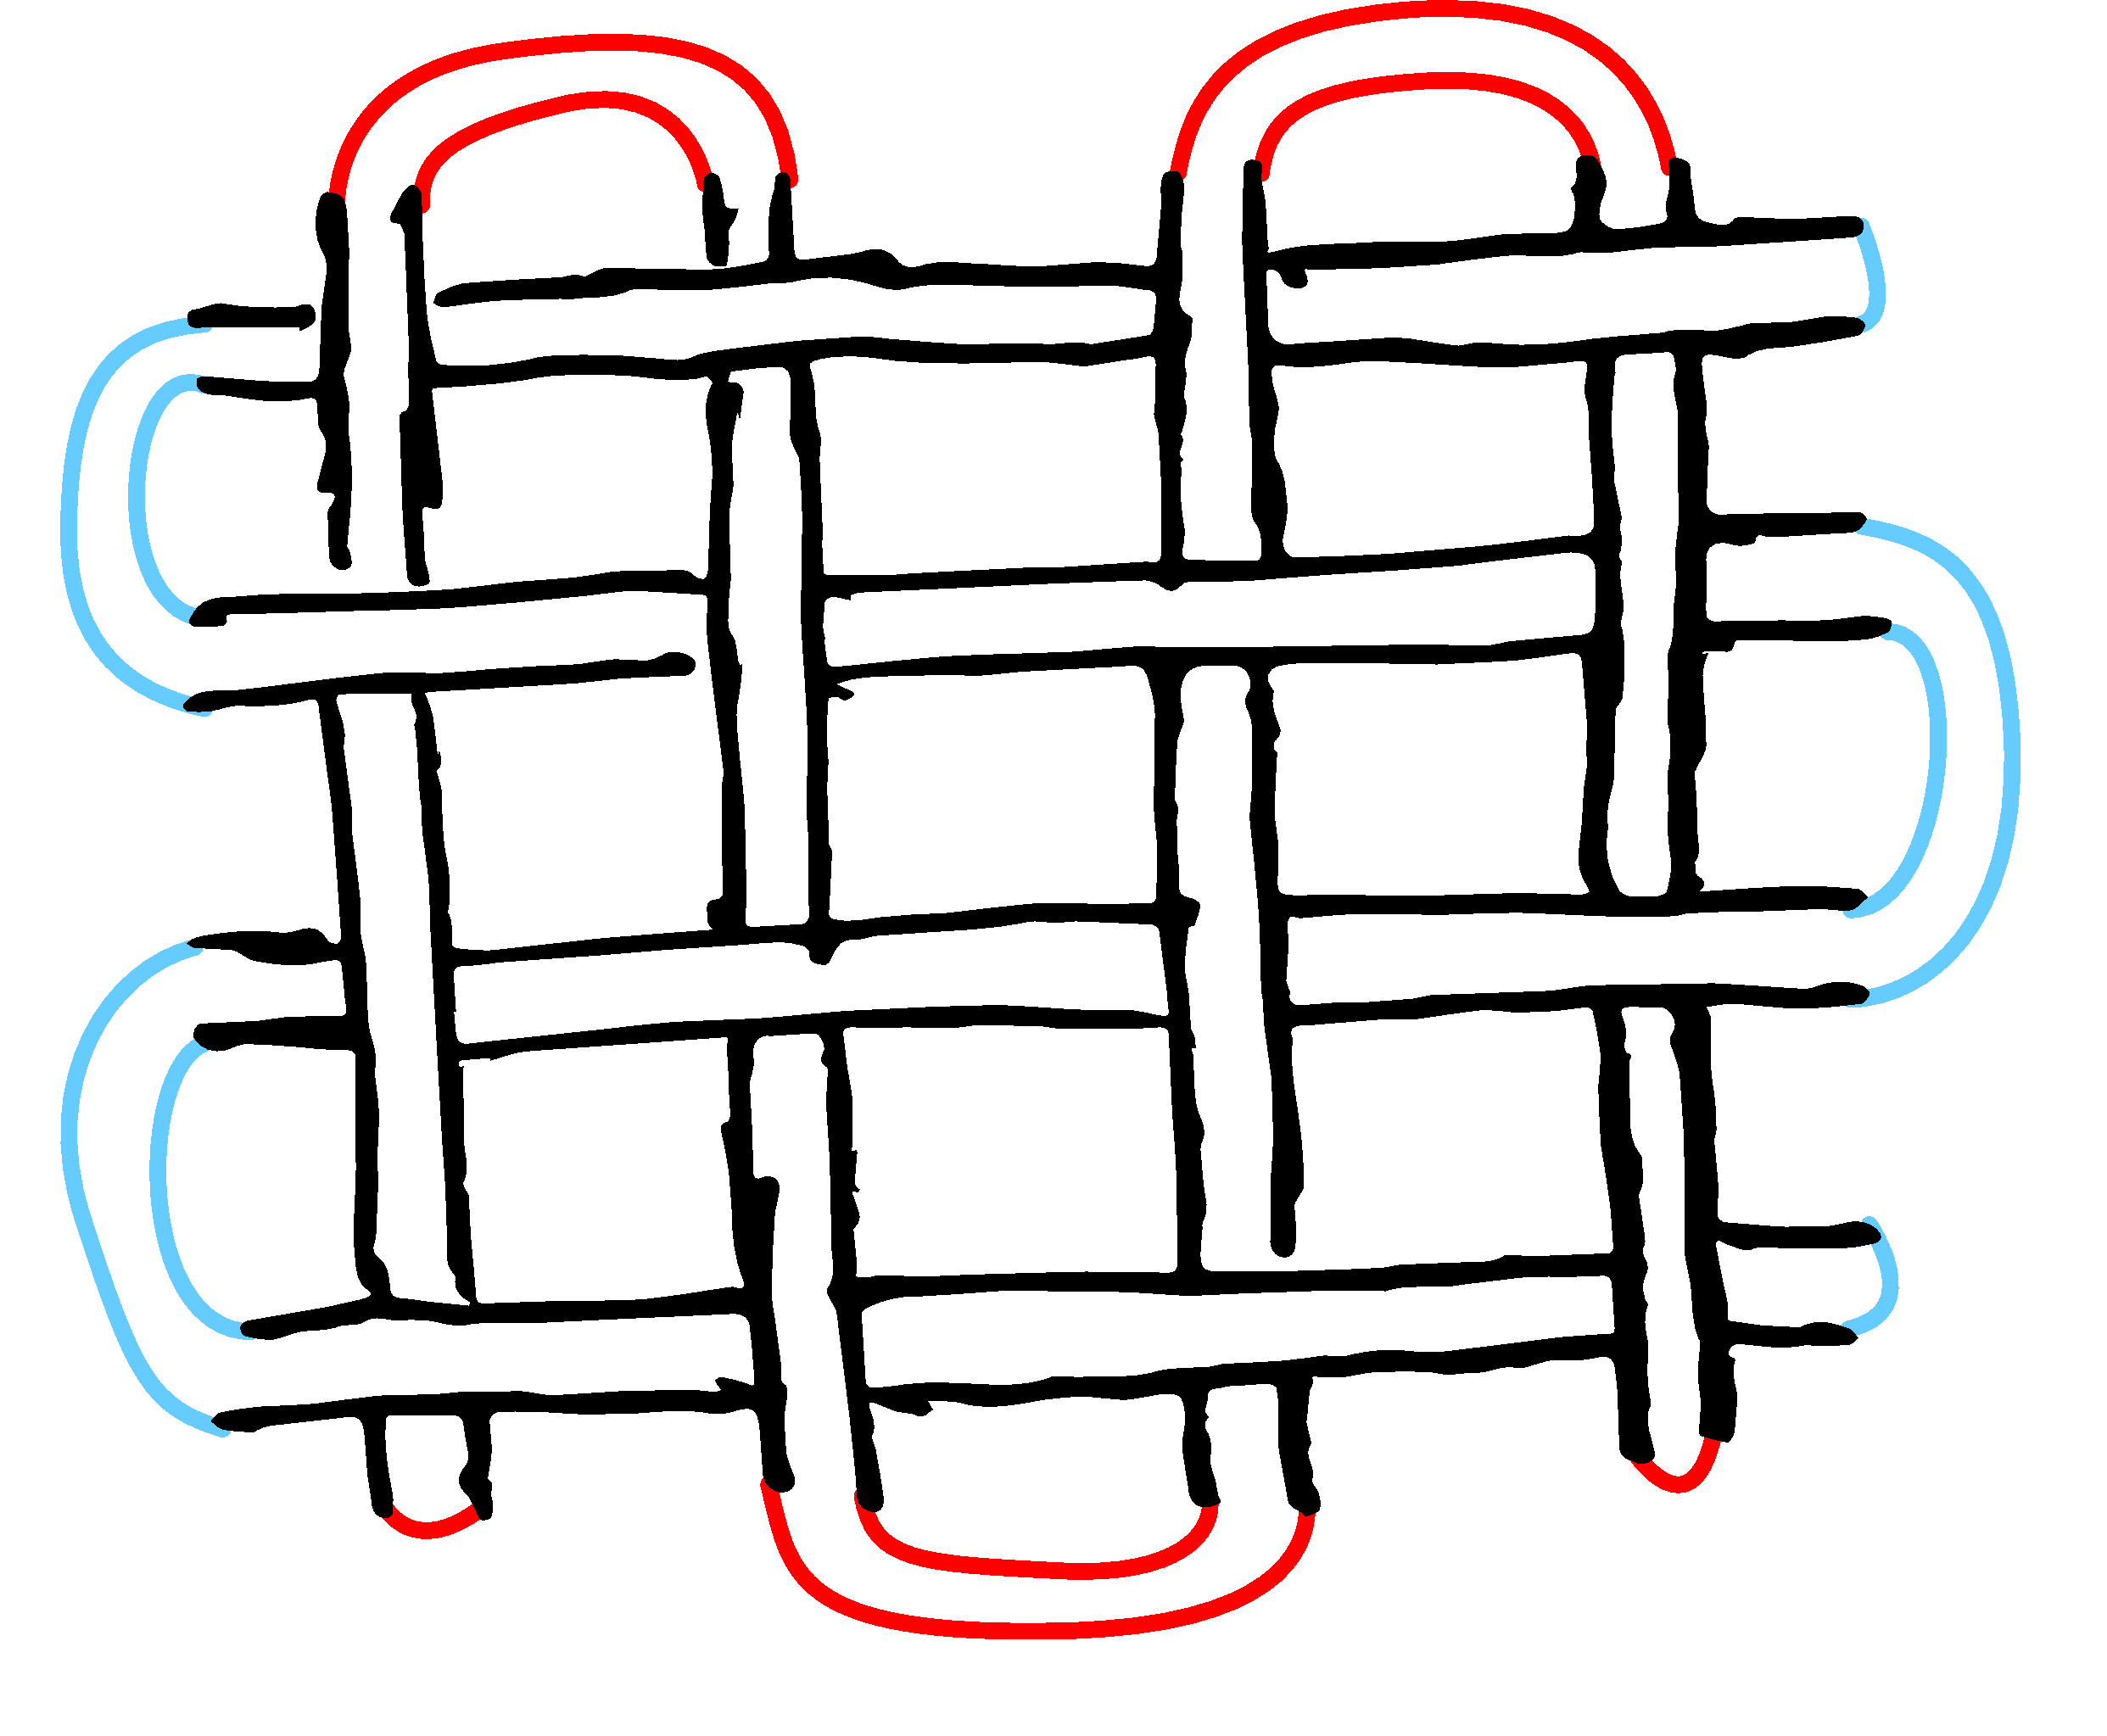
\includegraphics[width=0.3\linewidth]{figs/UF_weave_contweftwarp.pdf}
    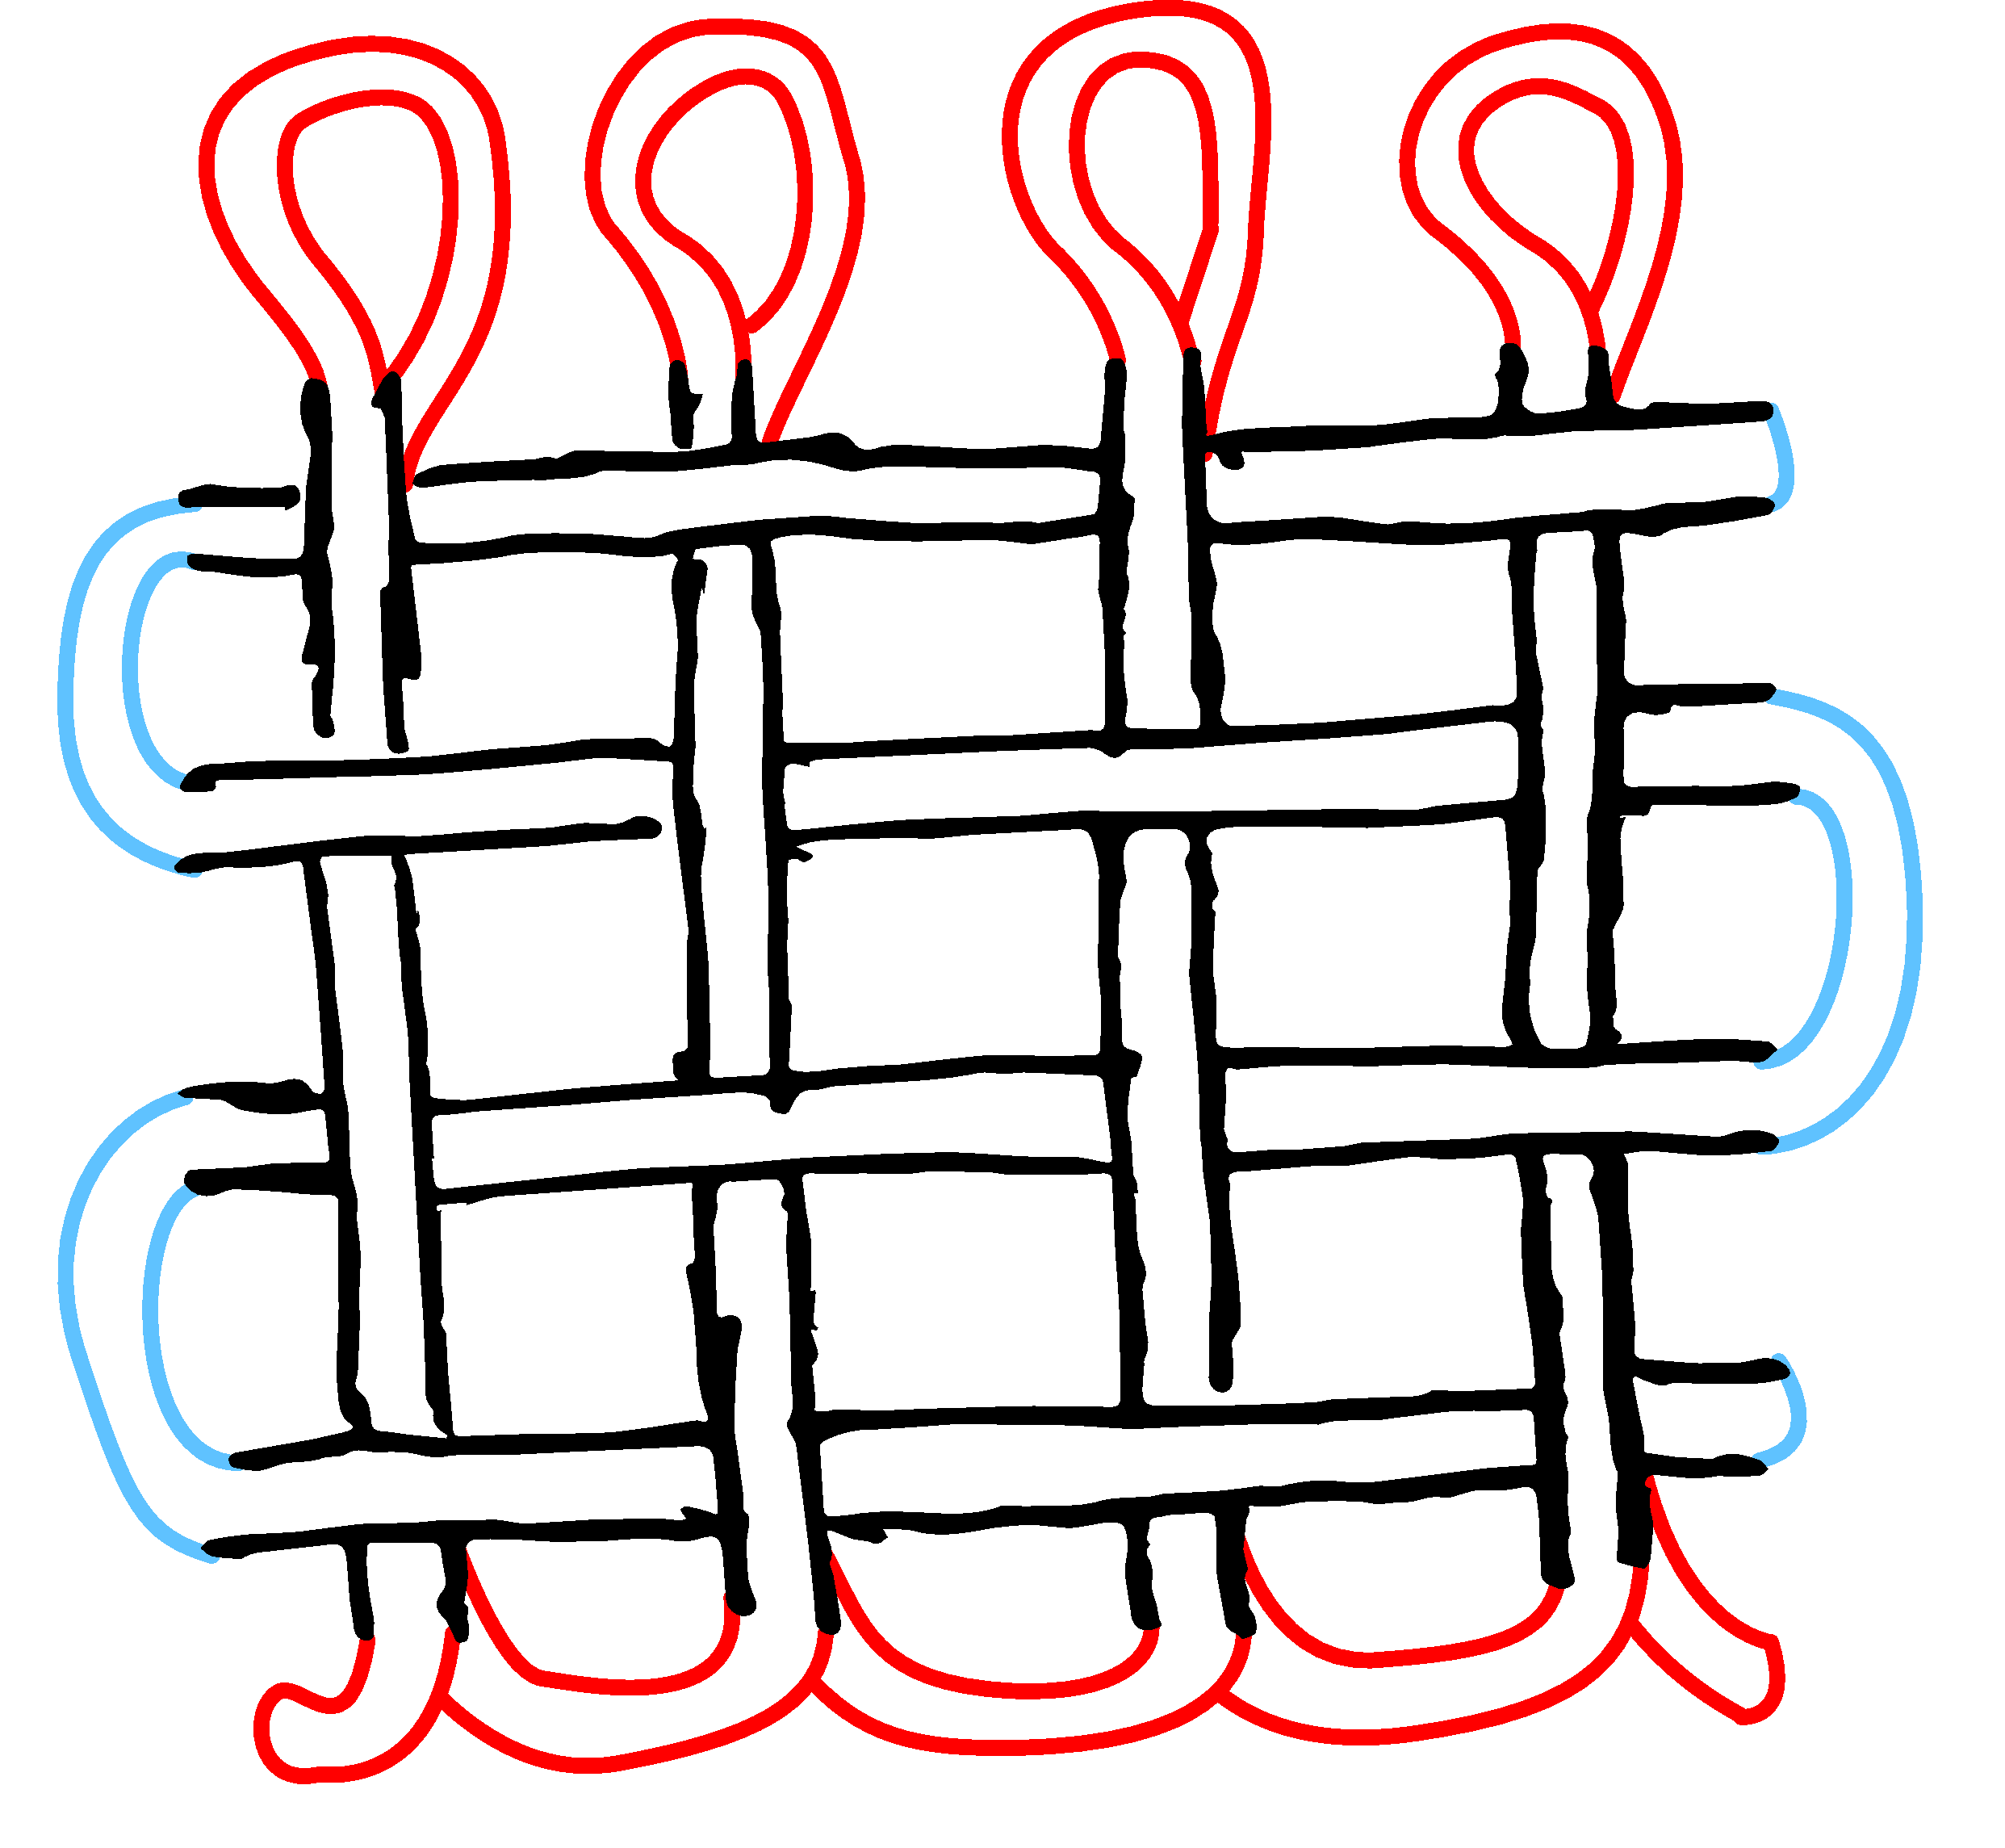
\includegraphics[width=0.3\linewidth]{figs/UF_weave_contweftwarp2.pdf}
    \caption[Unravel-able weaving experiments.]{Diagrams of the three warp securement experiments. (left) experiment 1's method of continuous weft and tying the cut warps, (middle) experiment 2's method of adding one long continuous warp, (right) experiment 3's more successful method of "pairing" each warp to support quick disassembly}
    \label{fig:warpDiagrams}
\end{figure}

The following sections describe three experiments we conducted to maximize harvestable yarn while supporting shape weaving.

%include a figure or table here to show details of each technique
\textbf{Experiment 1: Continuous Weft \& Bound Warp:} In the first experiment, we  kept the weft yarn continuous, cutting the warp and knotting the ends of the warps in small bundles to secure the shape. While this would be fairly easy to implement on a larger loom without any modifications, this knotted warp method did not address warp yarn wastage as the warp would still be cut during finishing. Furthermore, it would be extremely time-consuming to tie hundreds or thousands of knots in a larger piece (Figure~\ref{fig:warpDiagrams}, left).

\textbf{Experiment 2: Continuous Weft \& Supplemental Continuous Warp:} In the second experiment, we explored using a continuous warp as well as a continuous weft to further reduce wastage. This sample was woven on a small sampler loom, where simple pins supported each bend in the warp yarn. %{a quick sentence on your loom setup for doing this}. 
As seen in Figure~\ref{fig:warptightening}, this modification allowed the excess warp to be tightened against the shape's edge. After weaving the shape, the weaver takes each loop of excess warp and tightens it against the edge of the piece, locking the weft yarn in place. This selvedge (self-edge) technique creates a finished, secure edge without any further cutting or sewing. However, this continuous warp method would be difficult to scale to more complex looms, as the continuous warp would have to be manually threaded through several components within the loom (Figure~\ref{fig:warpDiagrams}, middle).

\begin{figure}
    \centering
    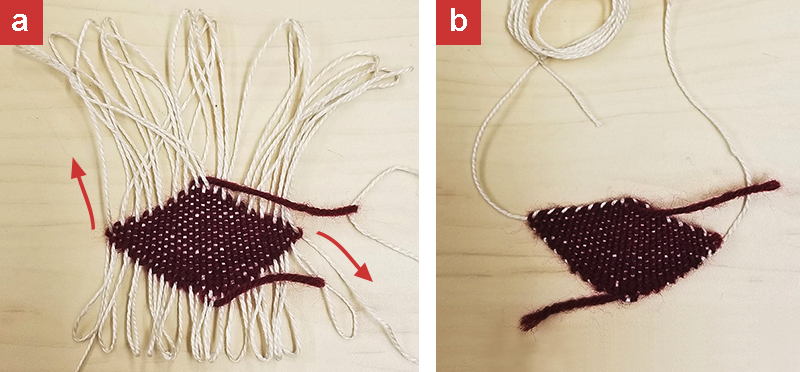
\includegraphics[width=\linewidth]{figs/UF_warptightening.png}
    \caption[Before and after photo of a warp-tightening method to facilitate shaped weaving.]{Modifying the woven structure to facilitate future disassembly with a continuous warp. a) The warp is initially in a rectangular area, with the weft filling the desired shape. b) The weaver tightens the warp to lock in the edges of the shape, leaving long ends of warp at either end of the piece. While this represents some waste, it is much less waste than generated by cutting the wefts, and warp yarns are often a natural, abundant material such as cotton.}
    \label{fig:warptightening}
\end{figure}

\newpage
\textbf{Experiment 3: Continuous Weft \& Doubled Supplemental Continuous Warp:} Our third and final experiment continued with the idea of continuous warp, but with the warp yarn doubled on itself in a series of loops. Each looped pair of yarns was handled together in weaving (meaning that each paired warp would be lifted or lowered at the same time, just as though they were a single thread), and a final \emph{catching row} was inserted through all of the loops. This essentially creates a rectangular shape with a long continuous warps bound at the top by a catching row. To adapt this structure to the variable shapes of weaves (which may not be rectangular), we developed a process to tighten the warp, a variation on the method from Experiment 2. This is accomplished by pulling the ends of the continuous warp until it the warps and catching row conform to the boundary of the woven shape. This method results in a woven fabric which can unravel quickly once the catching row is pulled out of the edge. Furthermore, {while there still remain several barriers to scaling to industrial weaving,} this last method seemed \textit{possible} to scale to a larger piece on a more complex loom. %\todo{Continuous paired warp was the most successful, so exploring how to expand that to a larger piece - physical mechanisms? Computational design tools? Designing a method to involve both human and machine}
For the remainder of our design inquiry, we used this doubled warp method for shape weaving in designing our smart textiles for disassembly (Figure~\ref{fig:warpDiagrams}, right).

\begin{figure}
    \centering
%    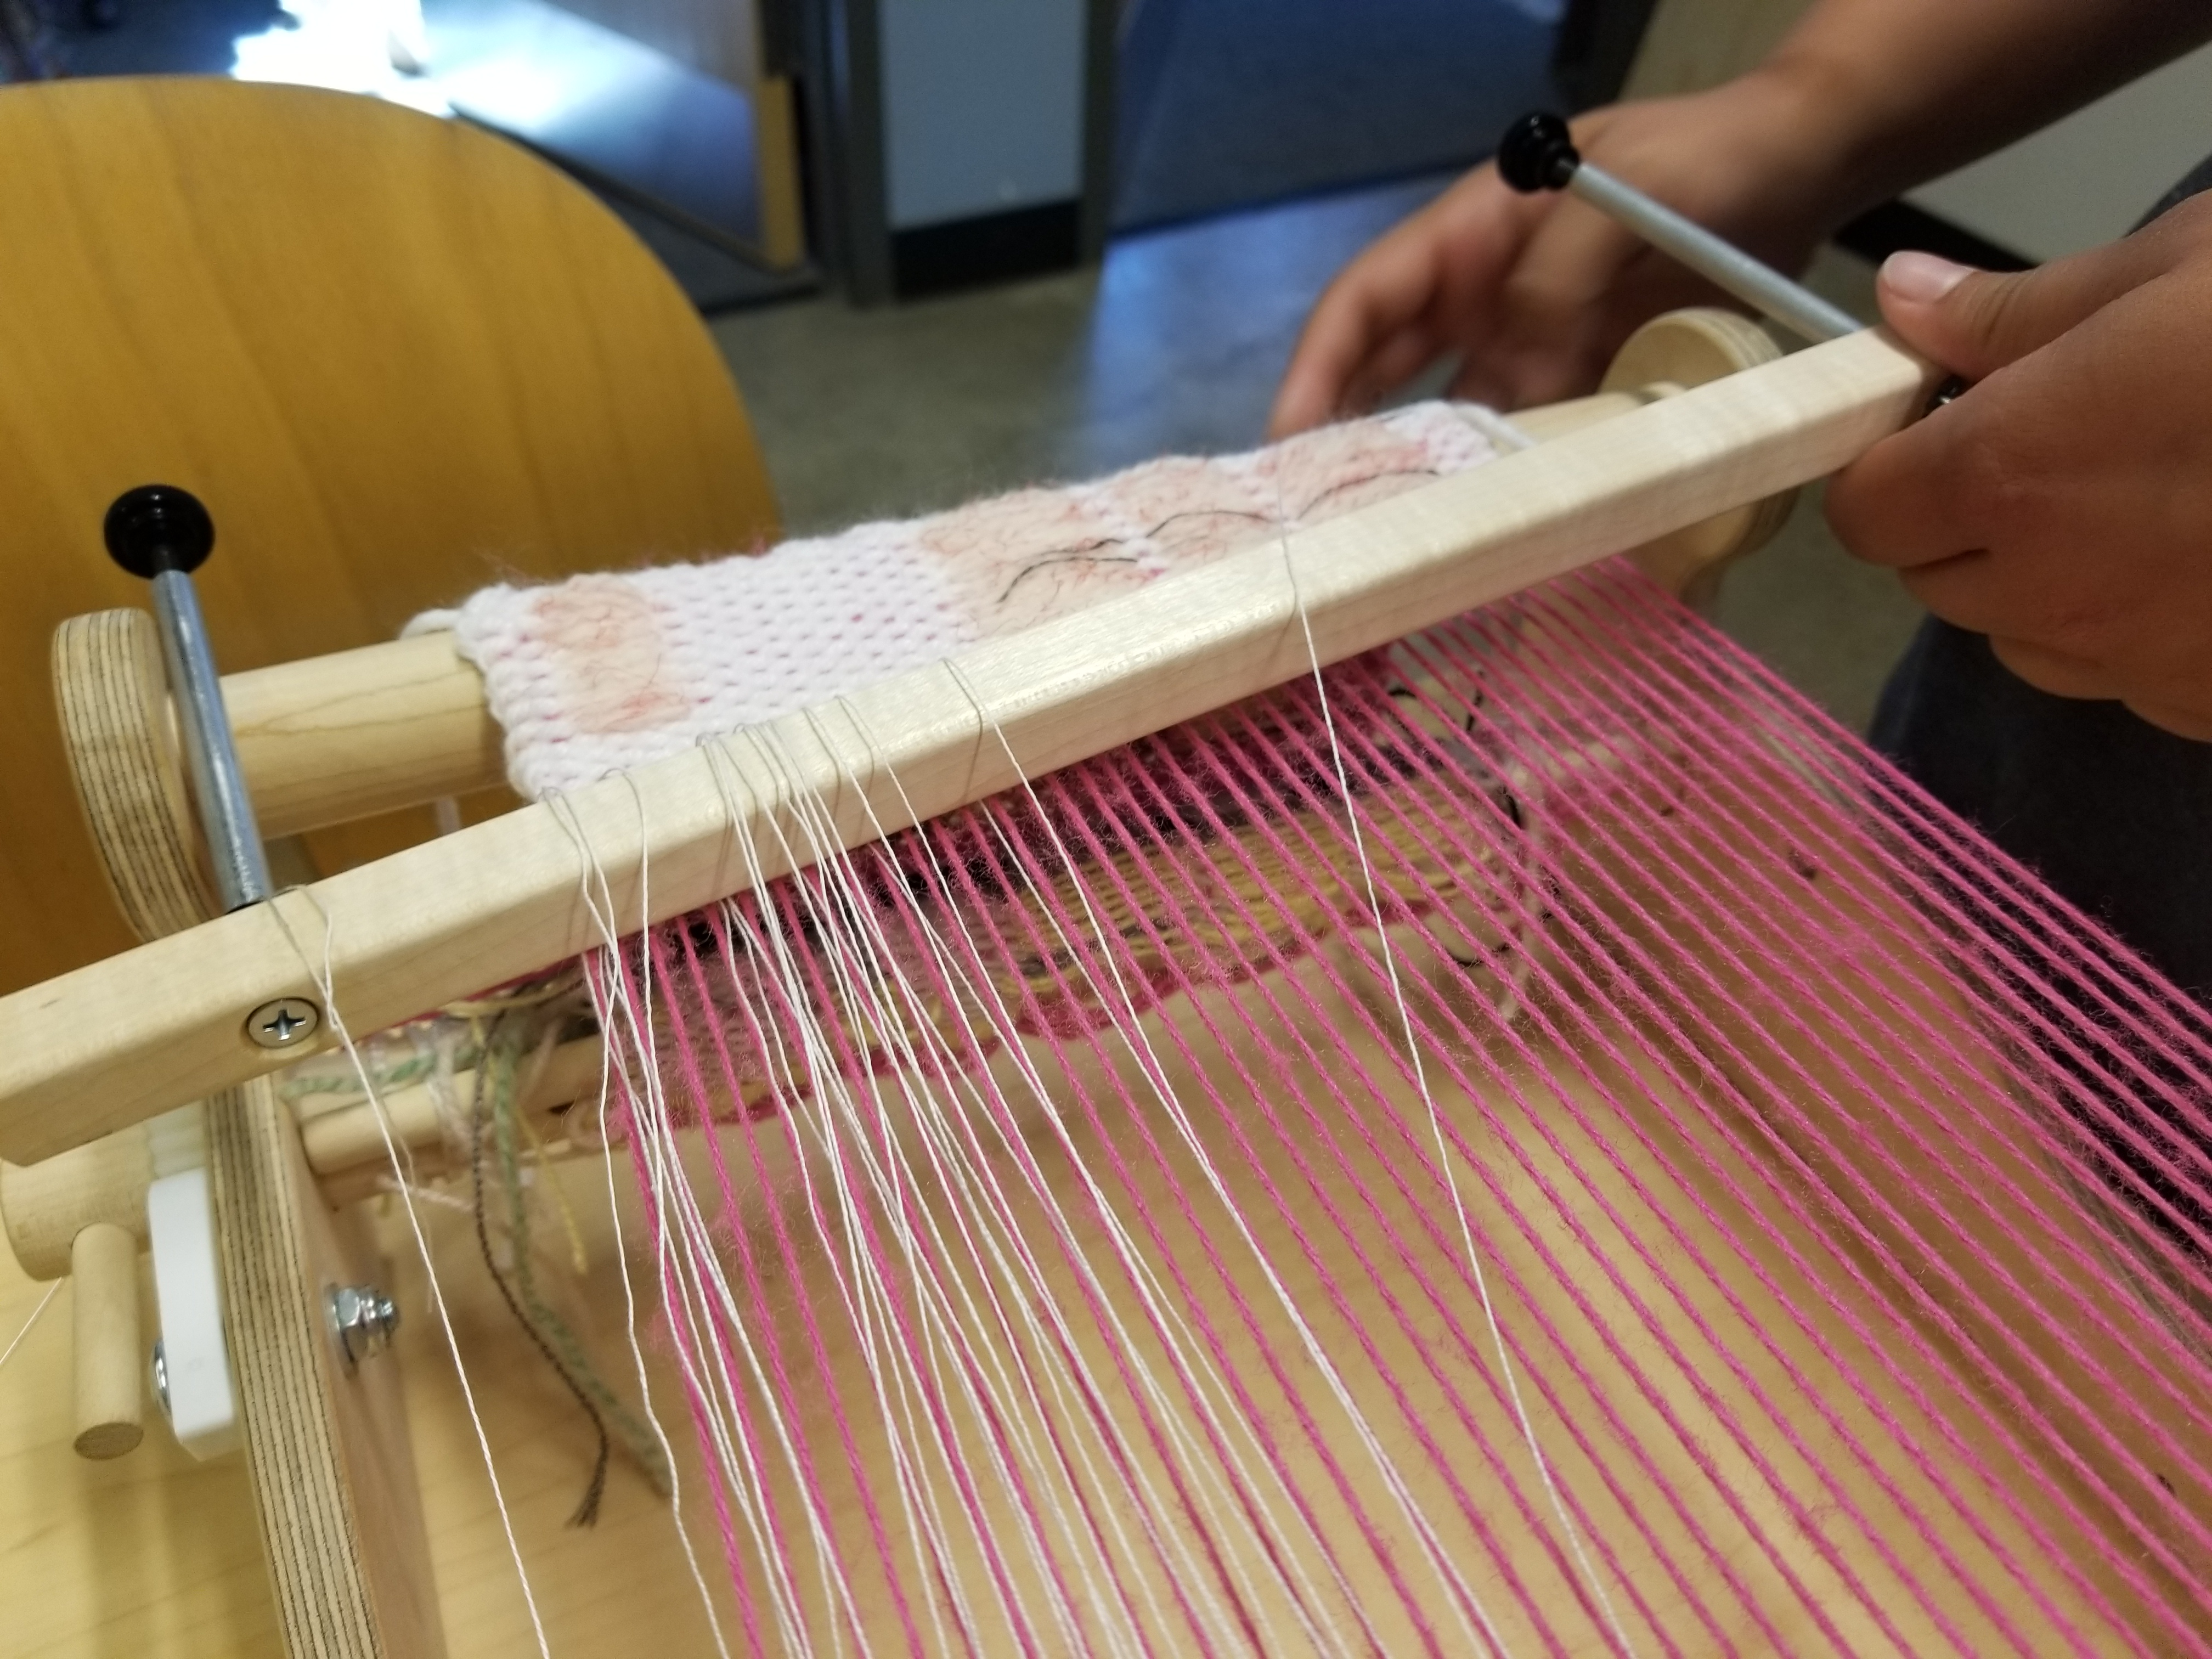
\includegraphics[width=0.8\linewidth]{figs/UF_loommod_inprogress.jpg} \\
%    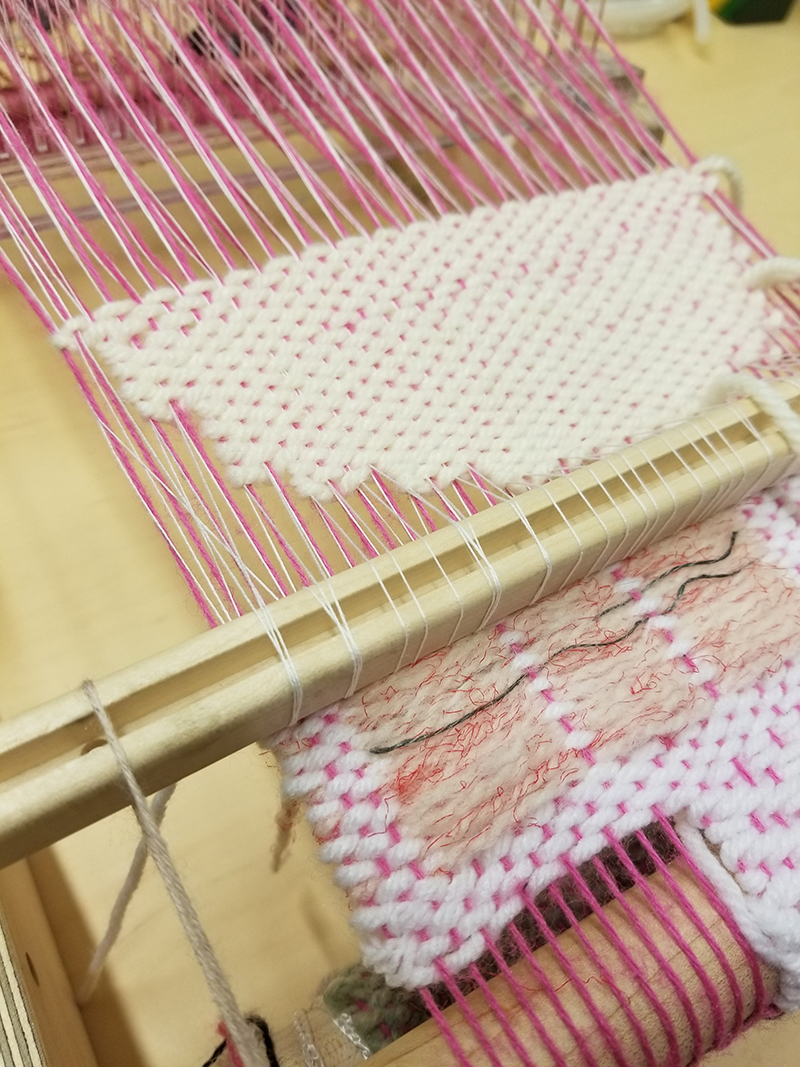
\includegraphics[width=0.4\linewidth]{figs/UF_loommod_front.jpg}
%    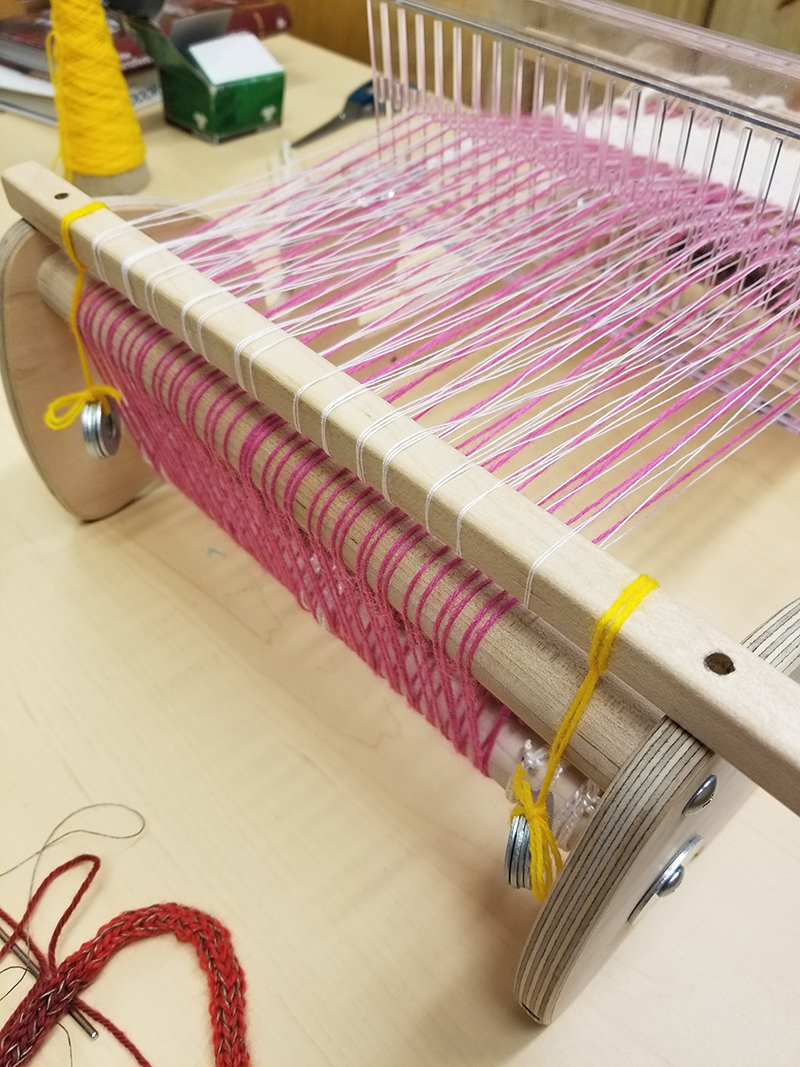
\includegraphics[width=0.4\linewidth]{figs/UF_loommod_back.jpg}
    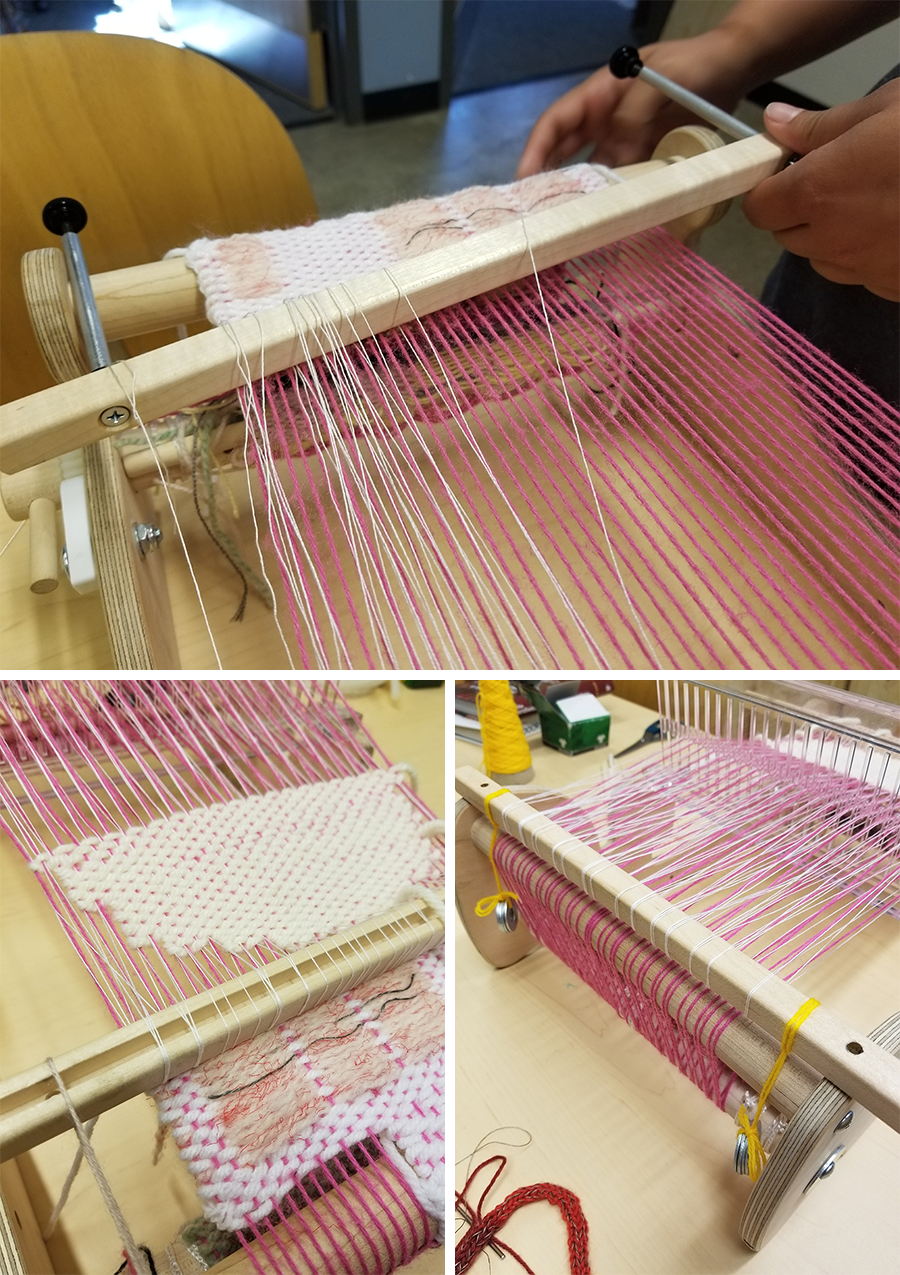
\includegraphics[width=0.8\linewidth]{figs/UF_loommod.png}
    \caption[Development of loom modifications for weaving unravel-able fabrics.]{(top) Developing new methods for maximizing the usable lengths that could be reharvested from woven fabrics required us to modify weaving equipment. These process pictures show how we inserted an extra beam into the loom to hold a modified warp (on top of the more traditional and existing loom warp). (bottom) The additional warp structure is created by adding additional beams secured in front and back for shape weaving with continuous warp.}
    \label{fig:loomMod}
\end{figure}

\subsubsection{Modifications to Physical Equipment}

We recognized that to weave larger shapes, such as garment pieces, we would have to adapt the loom machinery to accommodate our modifications to the woven structure. In order to hold the looped warp yarn during weaving, we had to insert additional beams at the back and front of the loom to maintain tension on the warps. Figure~\ref{fig:loomMod} shows the process and result of this modification. Adding beams to a loom has some precedence in other loom systems, where additional beams might be added to handle different tensions for multiple sets of warp yarns~\cite{essen_easysupp_2016}.

Equipment and physical tools shape the final product, and if the desired final product is not possible or easy enough with the current tools, it can often motivate shaping the equipment in return. The history of weaving and evolution of looms provide many examples of this symbiotic relationship between physical tools and craft object. For instance, many different looms, even a simple tapestry loom, can be used to weave velvet and other piled weaves \cite{essen_easysupp_2016}. During the Italian Renaissance, luxury demand for ornate, multi-colored velvet prompted weavers to develop specialized looms in which individual threads were weighted and dispensed separately \cite{watt_renaissance_velvet}.
Different types of looms encourage different weaving techniques and design challenges. In scaling a technique for higher-volume fabrication and disassembly, designing equipment includes trade-offs that can affect the values we want to express throughout the process and in the finished object. Industrial textile processes are \emph{not} optimized for disassembly and reuse. In fact, their optimization for assembly speed actually makes them much worse for disassembly.

This stage of material exploration informed later design tools to support such structures. By sampling several techniques quickly, we were able to see certain patterns in these techniques, such as how to secure the first and last few threads of each row when weaving. These techniques would later be implemented in our software tool as adjustments to the user-inputted draft. These experiments also directly provided insight into why knitting is easier to unravel than weaving: the fundamental structures of the two crafts impact their unravel-ability. 

% figure: screenshots of AdaCAD Shape visualizer
\begin{figure}[t!]
    \centering
    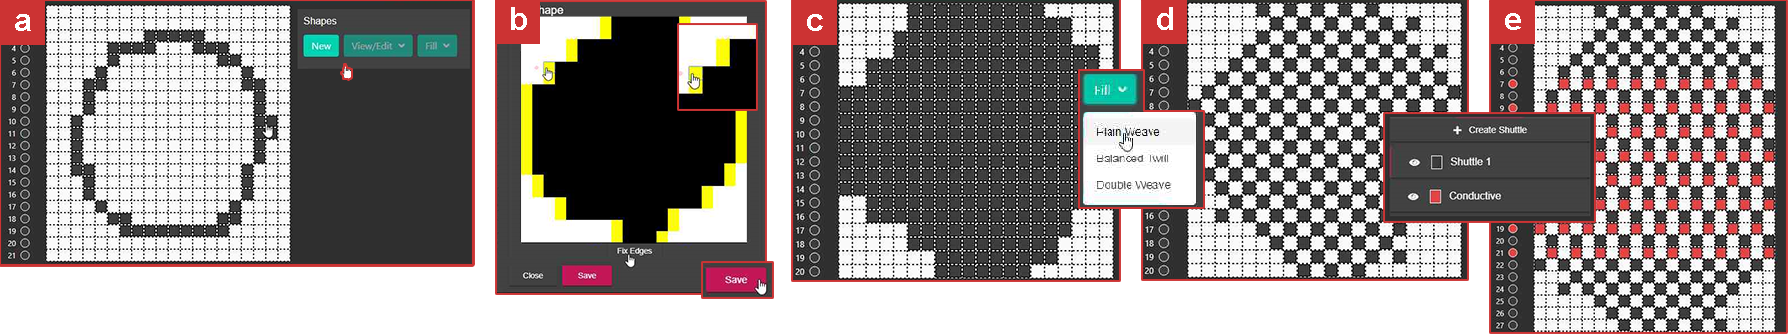
\includegraphics[width=\linewidth]{figs/UF_workflow.png}
    \caption[Example workflow for creating a shaped, disassemble-able woven smart textile.]{Example workflow of creating a shaped smart textile using the Shape interface. a) initial sketch of the piece's shape. b) editing the shape and refining its edges according the yarn constraints. c) changes reflected in draft view. d) filling the shape with the desired woven structure. e) adding conductive yarn to the design.}
    \label{fig:draftDesign}
    % \vspace{-1.5em}
\end{figure}

In designing and weaving these woven shapes, we had to consider both the desired shape and the fabric structure simultaneously. This process was unlike creating a swath of fabric, then cutting out a shape. Yet it was equivalent to weaving a shaped piece of a garment. We realized that cut and sew garment-making lends itself to selecting the fabric apart from the garment's construction. In contrast, a fully fashioned approach is a more tightly integrated process where the maker must consider the fabric's and garment's properties simultaneously. Thus, the garment emerges earlier in the design process.

\subsection{Encoding Practices in Computational Design Tools}

The weaving draft has long been in use as a machine-compatible format to communicate woven designs. Our previous work in AdaCAD combines features of different CAD practices to support integrated woven textile and circuit design~\cite{friske_adacad:_2019}. The program provides a basic toolkit for editing drafts on a canvas, making visual patterns, textured stitches, and rectangular structures easy to insert into the design. To better support shape weaving, we incorporated findings from our weaving experiments into an extension of the software. While we specifically made an extension in AdaCAD, the features could be integrated into any program that manipulates weaving drafts.

\subsubsection{Shapes from a Draft}

The key feature of this shape weaving extension is the addition of the Shape structure in the program's model of a woven design. AdaCAD models the draft as an array of booleans, and previously did not track any higher-level details about the draft outside of which yarns were in use. While a user could create a structure (e.g. a pocket) and visually see the area on screen, AdaCAD would not be aware of which patterns or structures were in the draft.

With the extension, the draft can have Shapes linked to it, storing information about where each Shape is located on the design. Each Shape is defined by the shuttles or yarns used to create it and stores the exact bounds of each row of yarn. Since the Shape tracks its exact placement in the draft, it can edit the draft appropriately to ensure the edges are secure. Furthermore, since the Shape tracks which yarns are used and the lengths of each row, we can now also calculate the amounts of yarn used in each design to support working with limited materials. By adding these data structures within the draft, we created a layer of abstraction between lower-level fabric details and higher-level shaping.

Figure~\ref{fig:draftDesign} shows an example workflow through the software from a users perspective.

\subsection{Design Artifact: Shape Woven Soft Potentiometer}

% Description of artifact
To encapsulate the various techniques and tools developed in our method for unravellable smart textiles, we created a proof-of-concept woven electronic component designed with our software tool. We decided on a circle for its symmetry, as well as the technical challenge of creating a smooth curved edge in a low-resolution medium. This component uses the doubled warp technique described earlier ~{(and depicted in figure~\ref{fig:warptightening})} to create its circular shape. The weaving incorporates a resistive yarn in an half-ring region, which allows the component to be used as an analog input (e.g. a position sensor or soft haptic slider). This particular resistive yarn also served as an example of the precious nature of conductive yarns and other emergent materials. Our lab had obtained a single sample of the yarn from a now-defunct mill, and we have not been able to source it or a replacement since.

To create the Smart Circle shown in Figure~\ref{fig:smartCircle}, we used the shape weaving interface in our software tool to generate a draft. Starting in the initial canvas, we sketched a circle that filled the width. Then from this outline, we converted the region to a Shape, which allows us to refine the edges in a separate dialog and fill the Shape with the desired stitch or woven structure. Once this Shape established the foundation fabric, we then designed the sensing regions by creating new layers in the draft via the Shuttles menu. 

Once the draft was prepared, we exported the file as a bitmap image for future use in a computerized loom. We then printed a large version to execute manually on a simple loom. This particular component was woven on a rigid heddle loom, a small, beginner-friendly loom that is also used for sampling by experienced weavers. Regardless of the type of loom we chose, the shape weaving required us to set up a continuous paired warp as previously described. This smart textile component, by incorporating the various elements of a designed-for-disassembly method, demonstrates how such a method is a combination of learned procedures, physical infrastructure, and computational design representation in a draft. 

\begin{figure}
    \centering
    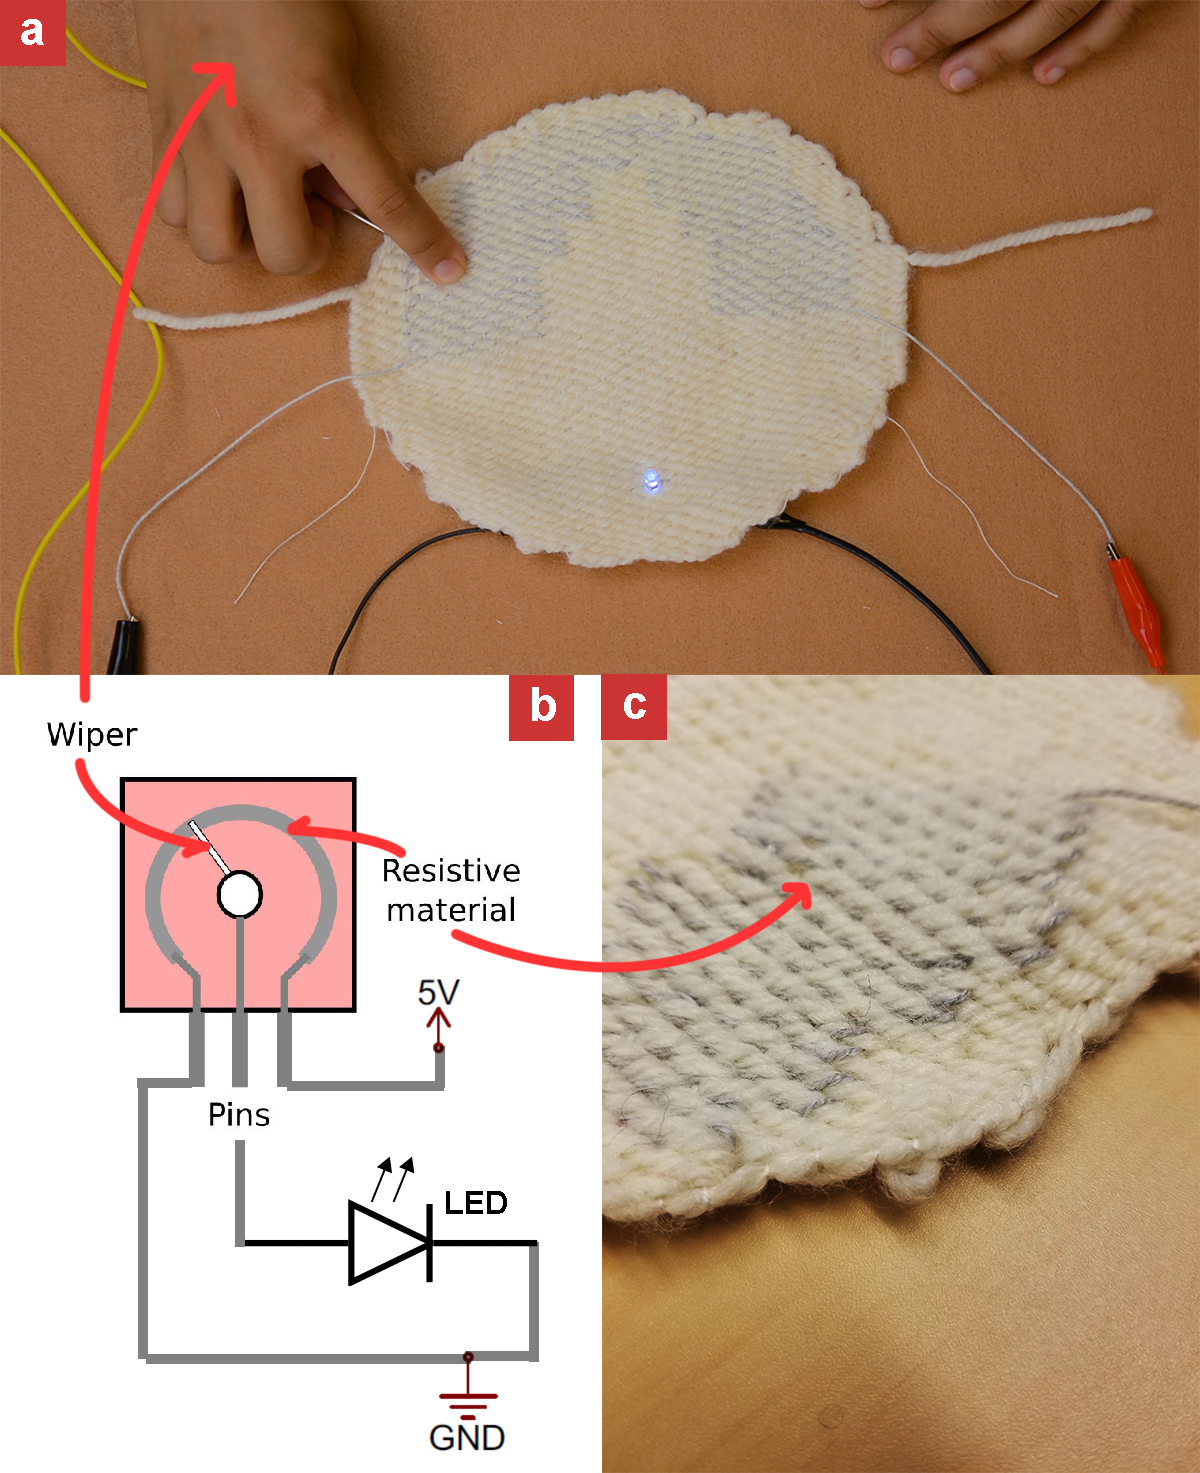
\includegraphics[width=0.9\linewidth]{figs/UF_sensor.png}
    \caption[Prototype of a smart textile potentiometer component.]{a) Woven Smart Circle component in use as an analog input in a circuit. b) Diagram of potentiometer controlling an LED for reference. c) Detail shot of integrated conductive material and the piece's finished edges.}
    \label{fig:smartCircle}
\end{figure}

We connected the Smart Circle to a simple position-sensing circuit. While this interaction and type of voltage-dividing circuit is fundamental to many systems, the textile nature of the Smart Circle suggested new designs for us. The texture of the sensing region was hard to distinguish from the soft ground fabric, and even the visual impact of the resistive yarn was subtle. Aesthetically, we could imagine woven smart textiles with invisibly integrated electronic components that are designed for disassembly. Not only could sensing within the fabric operate on hidden mechanisms, but the invisible doubled warp and other disassembly techniques would conceal the untold story of the smart textile's fabrication. Only when a hand touches and works with the object, are its secrets revealed.

The Smart Circle took about 1 hour of set up, 2 hours of weaving, and less than 15 minutes to unravel. The only waste from the fabrication and un-fabrication process was a yard of the abundantly-available cotton warp yarn which we trimmed after tightening. We recovered all of the precious resistive yarn. The time that we put into design and fabrication was not wasted---rather, we recovered the time. The yarn used in the Smart Circle will be used in the future for many more hours and prototypes.

\section{A Design for Disassembly Provocation}

Having explored designing smart textiles for disassembly along one route, we now invite other researchers to explore the space in their own ways. Through our work, we found the process of designing to benefit from both technical explorations paired with sensitizing exercises. The unraveling/sensitizing exercises were useful for grounding the design principles in existing practice and conventions above privileging a solution that was specifically "novel." Furthermore, it gave a more embodied sense of the time that is currently involved in undertaking disassembly.

A process that incorporates disassembly from the start might change our relationships with time during fabrication. Our shape weaving interface (and the entire process) forces the maker to slow down and use their time and work with the material. Disassembly functions as a challenging constraint to consider within this process. %While we believe this time-slowing provides a broader space for considering the materials to be used, we also see opportunities for leverage computational processing to optimize patterns based on heuristics that maximize each yarn length.
Pairing these sensitizing and reflective practices in parallel with augmenting our software and hardware tools helped us see the tension points with existing equipment and infrastructures of textile production. %Fashion designs are accustomed to having the ability to select a fabric prior to construction. These loose sheets of movable fabric are central in processes like draping. 
While the tools we provide will necessarily limit the design space and the creative approaches, they might also provide new and unexpected aesthetics, such as unusual seeming patterns that emerged from a computationally generated sweater \cite{beta_brand_brown}. In this section, we discuss these themes that emerge not only in our work, but also other perspectives in sustainable HCI and computational design.

%Also, considering the assembly design can affect not just how different stages take shape, they are manufacturing methods but also design choice and that the way the bring different elments of the garment into, as such, the garments emerge earlier the process. So if one way to design for sustainability and sustainability is to entangle multiple factors, then one should slow down to give each relationship enough time. The following action items in this section all relate to slowing down.

\subsection{Shift from Throughput to Longevity}

The efficiency of manufacturing is generally measured in terms of throughput, the quantity of material or goods produced per time. What if we defined efficiency as how long the material can last? We might aim to maximize longevity: the amount of time a material (independent of its object form) stays useful. Dew et al.'s 2019 work on crafting with waste material from makerspaces highlights how this question may not only help us reflect on waste-producing processes, but also imagine new ways to salvage materials from being ``unusable" \cite{Dew:2019:DWS:3322276.3322320}. Shifting this argument from human actions to the tools complicit in these actions, we see that many design tools and fabrication machines could better support longevity in the materials we use. Could our tools and machines support continuous materials, disassembly, and reuse by default? The modification of physical mechanisms and design tools in tandem illustrates that this is a challenge to be addressed through multiple channels, including design and manufacturing. 

We believe that this shift need not create more difficult processes. By designing tools to support disassembly, other values can bubble to the surface when we anticipate care and maintenance, rather than disposal, during design and fabrication. Craftspeople describe a certain joy with working with the material and repetitive, meditative motions \cite{pye_nature_2007, fletcher_craft_2016, nitsche_when_2019}. Craft, especially contemporary craft which has shifted from subsistence to leisure, emphasizes joy and pleasure as a value in relation to time and labor. These craft mindsets are often compatible with ``slow" and sustainable thinking \cite{pan_fashion_2014, phelan_what_2017}. The more time a person gets to spend with the material, the more joy emerges during the process, and in the end, a higher-quality and longer-lasting product.

\subsection{Honor the Hands that Made the Materials}

Shifting the value of material production to quality time and longevity, rather than quantity and efficiency, could also reframe notions of production environments. Efficiency suggests a machine-dominated environment. As we see in commercial textiles as well as electronics, this is also an environment where human workers are invisible. We personally had the misconception that commercial textile production was largely automated, with human operators pressing a button on a machine. However, through unravelling, we saw that even industrial textiles still involve a lot of handcraft. Although the actual knitting or weaving is mechanized, textile production involves extensive human-machine collaboration, such as individually placing stitches on a linker and adjusting tension as the machine runs. \cite{engineers_complete_2017} Yet the hands are always there, in industrial processes as well as craft. 

As works in sustainable HCI show, humans will always need our hands to reckon with digital technology, and this manual intervention is more apparent in developing economies. For example, Jackson et al.'s Repair Worlds~\cite{jackson_repair_2012} focuses on maintenance and repair practices in Namibia's computing infrastructure, and Rifat et al.'s The Breaking Hand~\cite{rifat_breaking_2019} focuses on e-waste recycling workers in Bhangladesh. In more developed countries, this labor is hidden by layers of intermediary infrastructure, contributing to the environmental impact of globalization, to which Raghavan et al. proposes ``disintermediation" as a sustainability countermeasure \cite{raghavan_means_2017}. We believe that making manual work visible in the disassembly stages could further emphasize the hands that were present during assembly. What if clothes were designed for disassembly, and retailers encouraged the buyers unravel products themselves? This feature would be in line with design for disassembly principles, where disassembly is readily accessible and documented for any user \cite{webster_dfd}. Smart textiles products might include a ``pull here" tag to cue the unraveller into the process, blurring the lines between user, maker, and un-maker. We would hope that the increased visibility of the hand and its owner, the worker, would also lead to recognizing the value of their labor through improved labor policies in manufacturing. As consumer-users participate in the embodied craft of unravelling their own textile goods, they could individually engage issues of sustainability and repair in accessible, ongoing ways.

%\subsection{Try it Yourself, Notice and Attune, Then Design}

%In concert with a growing movement of DIY repair [CITE] %, and our own workshops hosted to bring people to experience their belongings in a new way -- not sure we should introduce this so late
%there are distinct benefits to doing the mechanical work yourself, as a sensitizing exercise, that you might typically ask someone else to perform or that you are assuming someone or a machine can do better. We considered programs of purchasing that require the purchaser or designer to perform all lifecycle stages prior to fabricating their idea. 

%Noticing and attuning - for designers of future systems. Based on the idea that textiles fabrication will continue to (re)grow in popularity. Designers might attend to slowness and care (Olly paper? Slow fashion?) as a sustainability tactic, embodying a different relationship with time, machines, and efficiency.

\subsection{Acknowledge the Histories and Futures of Materials}

Another consequence of industrialized textiles' high throughput is that most yarns, fabrics, and finished textile products are cheap and abundant. While there are luxury fibers, they generally have a cheaper alternative that functions similarly (e.g. warmth, tactile feel, visual appeal). However, with smart textiles research introduces new ``smart" materials such as conductive yarns, carbon nanotubes, etc. These materials are not only rare and costly to manufacture, but crucial to the textile's function. Wool and cotton were once just as labor-intensive to process, with entire communities spinning yarn from dawn to dusk to meet demand \cite{black_knitting:_2012}. These materials are \emph{precious}: expensive, scarce, and necessary to the design, and they need to be managed in their production and use. We could argue that with sustainability and post-growth \cite{fletcher_craft_2016}, \emph{all} materials are precious.

Continuing to recognize and work with the history of our materials may also change our perspective on novelty and progress. While in technology development, we may emphasize ``invention", craft communities have a term for (re-)inventing something that was lost or forgotten: ``unventing", recorded by famed knitter Elizabeth Zimmerman \cite{zimmermann_almanac_2012}. Many textiles craftspeople believe that there are no new ideas in techniques or tools in their practice, only new takes on old ideas. Rather than giving up on future work out of the fear that nothing is new, we can reframe this deep body of knowledge as fertile ground for new computational challenges. As Murer et al. noted in their design workshops on user interactions with deconstruction and ``un-crafting", designers may glean broader experiential values about their users and imbue their artifacts with deeper meanings if they design for disassembly as an intentional action \cite{Murer:2018:MTA:3196709.3196806, Murer:2017:UDE:3024969.3024993, Murer:2015:DID:2882850.2882860}. If smart textiles practitioners integrate the histories and futures of their materials into their design process, they would find many opportunities to engage with communities that have historically been labelled ``backwards" and to revisit supposedly-failed ideas that may simply not have received enough time.

%We seem to be looking for new computational challenges in fabrication. These tend to think of supporting user vision and creativity as reliant upon seemingly unbounded materials and powerful tools. But there is a suite of computational challenges to be studied from the perspective of blended users, makers, and unravellers.

\section{Creative Possibilities for HCI in Disassembly} 
While the practice of unravelling and disassembling is still emerging today, we can imagine a future where unravelling and reuse is an accessible and integral part of a smart textile's lifecycle, and perhaps even in other forms of technology. The Unfabricate experiments that we undertook revealed many possible concepts which we will explore with more samples and more rigorous analysis. To inspire future work, we present three distinct, yet intertwined threads of possible development, illustrated in Figure~\ref{fig:concepts}.

\subsection{3D Shape Weaving for Garments}

Our design artifact in this paper was limited to a single flat shape, but the design allows for future integration with other shapes to produce a full garment. Craftspeople such as Jacqueline Lefferts \cite{lefferts_fullfashionedweaving} and Holly McQuillian \cite{mcquillan2019hybrid} have demonstrated initial methods for approaching this challenge using a combination of computer aided design practices and weaving structures. We might also see promises in approaches developed by Tao et. al in "CompuWoven" \cite{tao_compuwoven:_2016}, which aims at producing 3D forms through basketweaving techniques. The paired warp method developed as part of this work could extend such practices to consider quick unweaving of "fully fashioned" woven garments.  A related extension of this work may also involve experimentation with linking mechanisms and other seaming techniques on shape-woven pieces. Using techniques from fully fashioned garment making will continue this work's dialogue with current textiles manufacturing processes, as well as fashion design.  For example, one could weave a sock heel or shoulder piece by weaving a concave flat shape on the doubled warp. When the warps are tightened, the fabric will naturally pucker and bend into a 3D curved surface. (Figure~\ref{fig:concepts}, top)

\subsection{Repairing and Modifying Yarn}

% While unravelling, altering properties (e.g. color, texture) of yarn as you wind it. Essentially an opportunity to re-spin or adjust the yarn. 
Unravelling presents an opportunity to renew the yarn of the original garment, beyond re-knitting or re-weaving the yarn into a new item. As the unravelling process involves winding the entire length of the yarn back onto a spool for reuse, the yarn could be repaired or re-coated as needed. More interestingly, one could re-dye or paint the yarn as it travels through the spooling equipment. (Figure~\ref{fig:concepts}, middle) For example, instead of using an inlay yarn to weave a figure, one could paint a yarn with segments of color that would then stack to form the desired figure. While this would be redundant with fabric printing for conventional dyes, this yarn painting method would offer much greater control for special smart textiles pigments, such as thermochromic pigments \cite{devendorf_adapting_2019}. Alternatively, painting the yarn with repeating color patterns would result in abstract, semi-randomized patterns emerging in the re-knitted or re-woven fabric, termed ``pooling" by handknitters \cite{plannedpooling}. Furthermore, in our software modifications, we saw that encoding more material awareness, specifically on yarn length and usage, allowed us to more precisely design shapes and figures. These modifications could be further developed so that future smart textiles CAD is not only aware of material constraints (e.g. a specific length of unravelled yarn to reuse), but could help the user work within such constraints to conserve precious materials.

%{Future AdaCAD Additions design with specific lengths of material (e.g. with shoddy?)}

\subsection{Modular Unravelling}
While this work was limited to completely unravelling a garment, there are design opportunities in supporting partial unravelling. Our shape weaving and supplemental warp techniques could be applied to select sections of a cloth, rather than the whole loom, to enable unravelling and replacing discrete patches or components. If a conductive component wears out, it could be removed, then repaired or replaced while leaving the base garment and the rest of the circuit intact. % connect to design for disassembly principles
Partial unravelling also recalls another practice in handcraft. In (hand) knitting and weaving, the crafts person can backing up a few steps, rows, or stitches if they make a mistake or want to modify the design. This reconfigurability means that the work in progress is not completely discarded as defective, as is the practice in manufacturing. If unravelling could be reframed as a continuous, natural part of the making process, it may suggest waste reduction strategies in designing textile manufacturing processes.

Together, these three concepts present custom-fitting garments, custom-painted yarn, and modular, easy-to-repair garments. One could imagine a future where smart textiles are nearly ubiquitous in our clothing, vehicle upholstery, and interior decor. Let us continue to speculate that all of these smart textiles are also designed for disassembly and reconfiguration. Not only would this future not have to contend with large amounts of e-textile waste, but humans could have an entirely different relationship with their textiles. A person could wake up in the morning, knit and weave their clothing and devices for the day, then unravel them in the evening. Rather than a closet full of clothes, they would have reserves of conducting and non-conductive yarn ready to go.

\begin{figure}
    \centering
    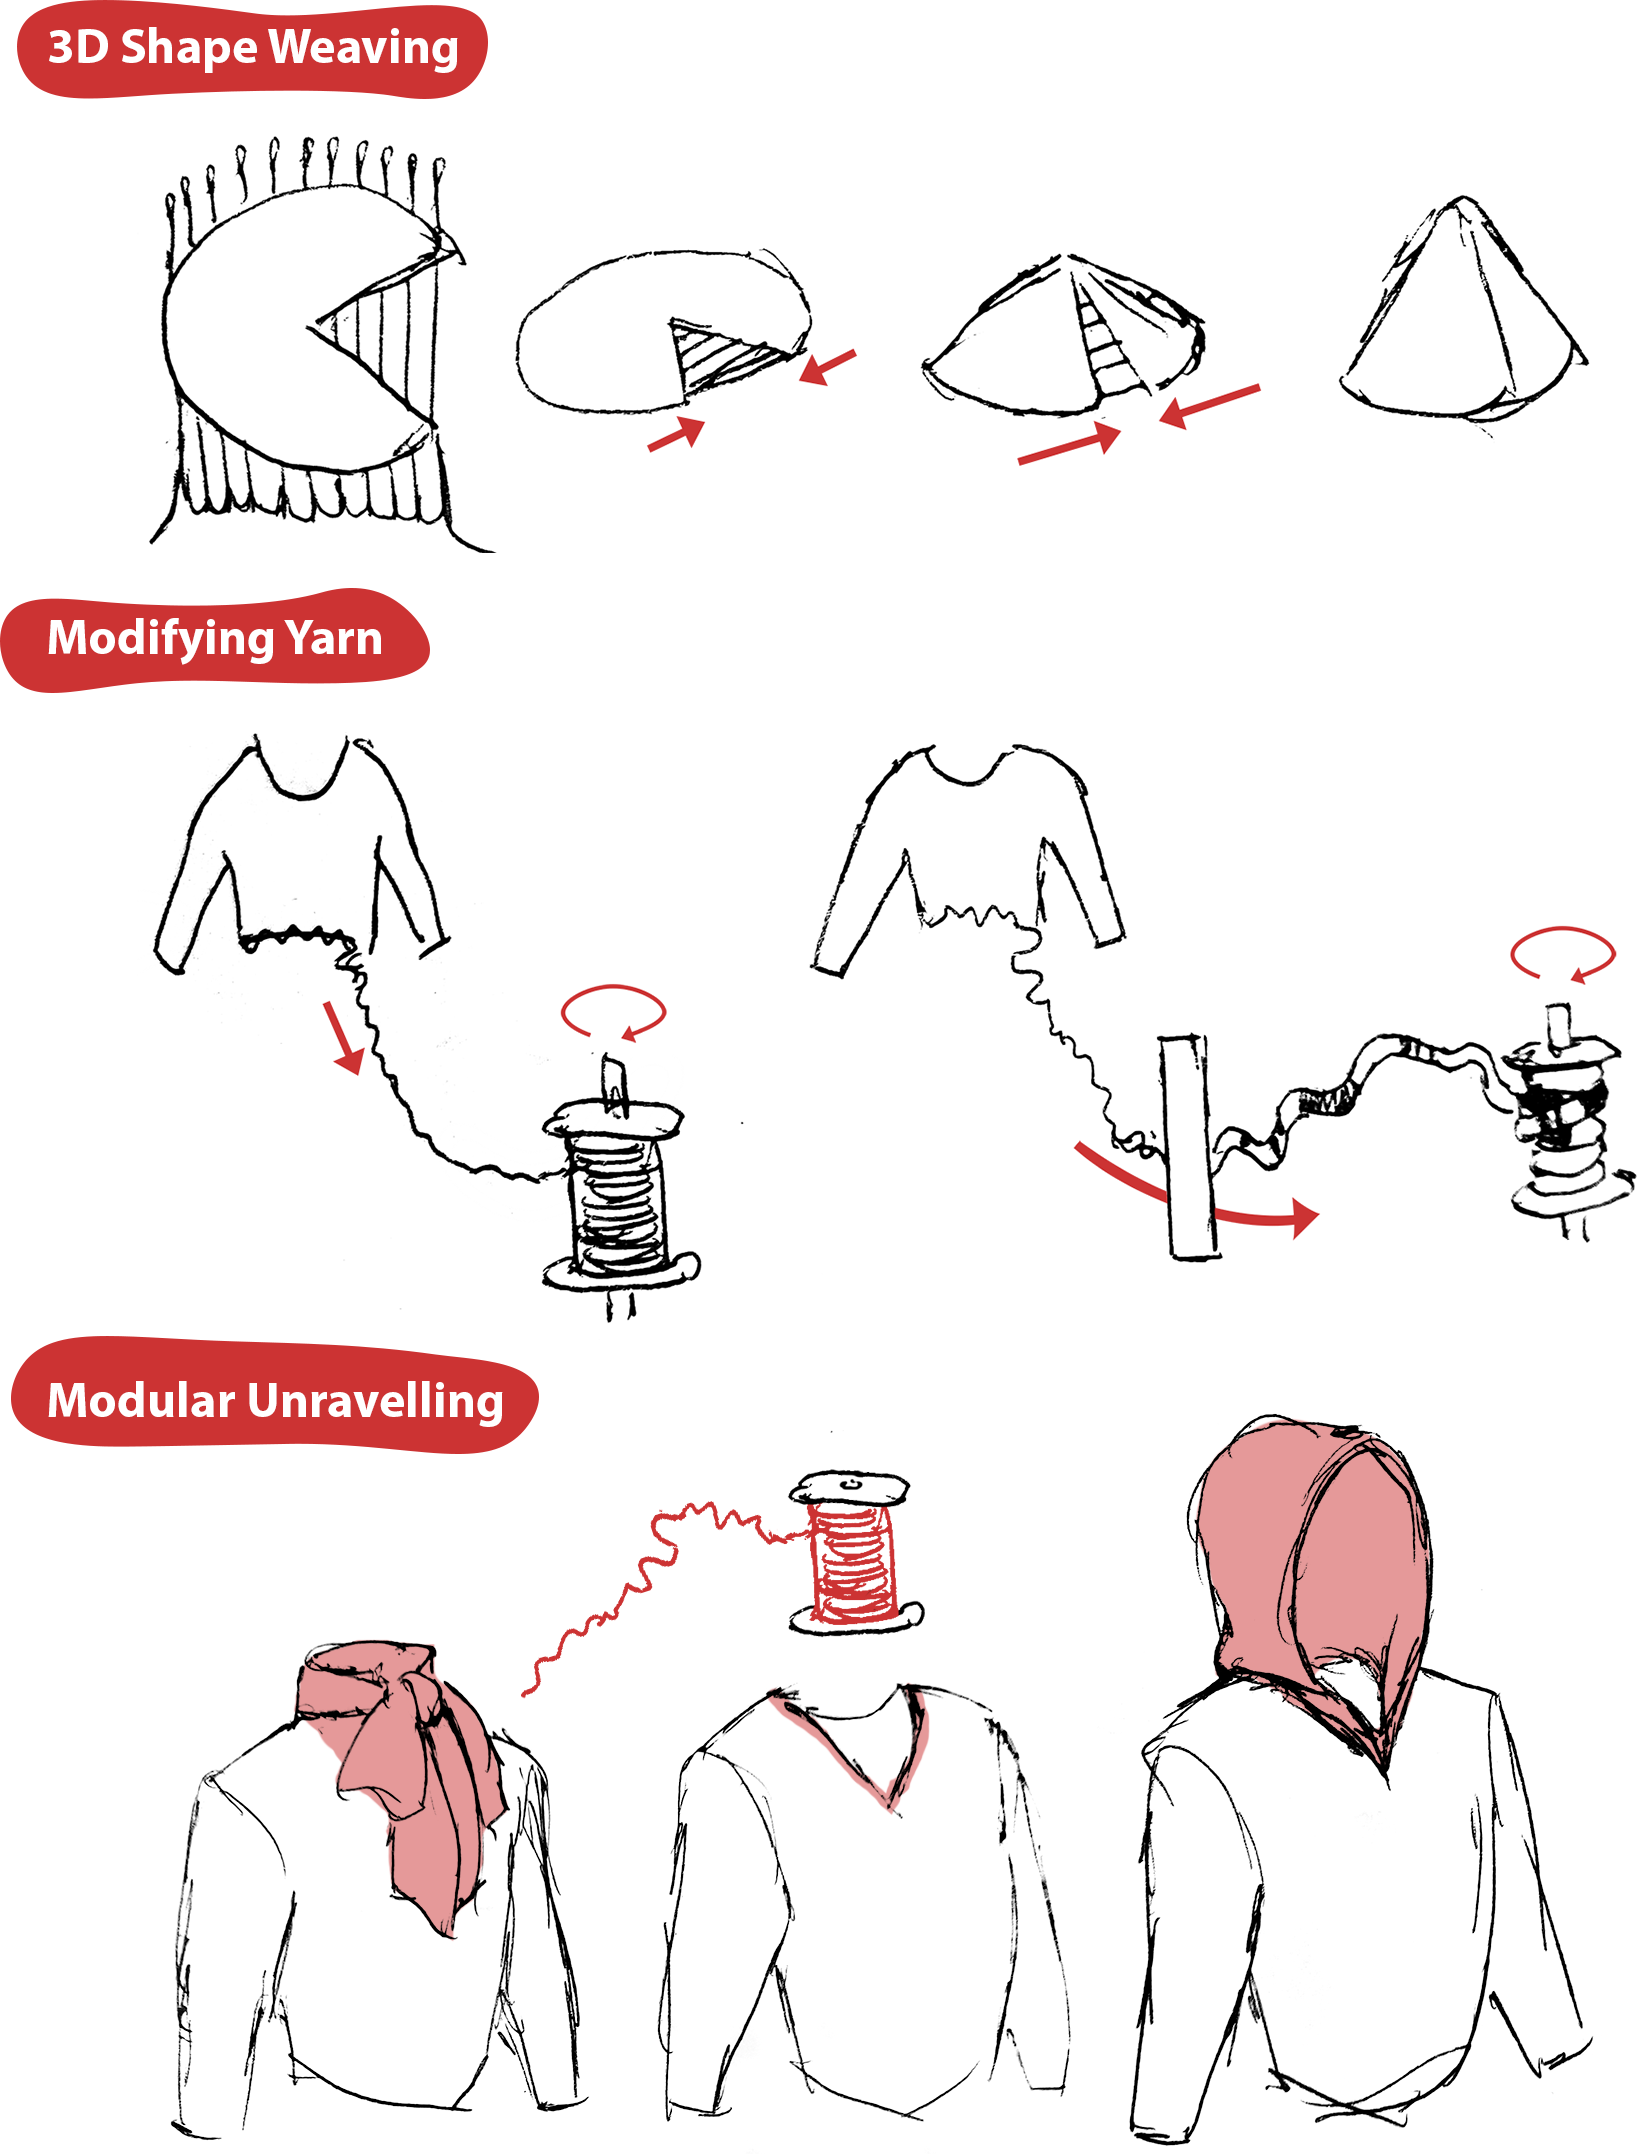
\includegraphics[width=\linewidth]{figs/UF_concepts.png}
    \caption[Three concept sketches in designing smart textiles for disassembly.]{Sketches of three concepts in designing smart textiles for disassembly. (top) Using the warp tightening technique to create 3D forms from flat, concave woven shapes. (middle) Introducing processes during unravelling which alter or augment the yarn. (bottom) Unravelling and remaking part of a garment to change its function.}
    \label{fig:concepts}
\end{figure}

\section{The Craft of Disassembly}

The idea of continuous fabrication, un-fabrication, re-fabrication evokes a possible smart textiles ecosystem of reusable, reconfigurable items. In pursuit of this future, we began a design inquiry to designing smart textiles for disassembly. Leveraging recent advances in computational design and textile-based fabrication, as well as existing properties of knitted and woven textiles that have existed for centuries, we were able to identify principles of disassemble-able textiles in both knitting and weaving to create interventions at design time to facilitate disassembly. We focused on weaving as the more challenging design space for disassembly. Identifying various modifications in fabric structure, physical hardware, and design software that could be made, we implemented a first proof of concept of a designed-for-disassembly smart textile lifecycle. Our work demonstrates how computational design inquiries can draw in other dialogues from materials science, fashion, sustainable HCI, and textiles engineering. We encourage other designers, users, and makers to also explore how to disassemble and reuse their future smart textiles. The smart textiles field uniquely lies at the intersection of two massive global industries, and leveraging textiles' physical properties and rich histories to design for disassembly could inspire a more sustainable technological sector. 

In thinking about the volumes of waste from both industries, I had an opportunity to engage with my ongoing interest in sustainability as a speculative value. As someone with professional experience in the fiber craft industry, I was familiar with contemporary practices among various crafters, whether they engaged for leisure or paid labor, including discourses around social values. Particularly in handcrafting textiles (in direct opposition to industrial textiles manufacturing), crafters often emphasize the value of slow, small-scale making and the direct involvement of human hands. Celebrating "slow" also directly connects craft discourses to several sustainably- or "green-" minded design domains, such as slow food, slow fashion, and slow technology \todo{[comps 52,105,111]}.

Anecdotally, after its publication in 2020, the Unfabricate project seems to speak to several different audiences. After presenting the work at a virtual Fabrication \@ CHI series in 2020, and being interviewed about Unfabricate (and other research) on a craft industry podcast, the Gist Yarns' Podcast, both crafters and HCI researchers alike seem to be intrigued by my "entangling" of craft and technology. The wide appeal of Unfabricate's conceptual premise may suggest that coproduction has potential as an interdisciplinary talking point, while retooling may speak to development patterns in many different technological domains. Yet in the end, Unfabricate left me with many open questions about scalability and feasibility with manufacturing. Without retooling as part of my research framework at the time, I did not have the language to directly engage with implementing systemic change from a manufacturing and process engineering perspective, nor from a design justice stance.